\documentclass[11pt]{article}
\usepackage{graphicx}
\usepackage{subfigure}
\usepackage{caption}

\usepackage{xr-hyper}
% this is for overleaf cross reference
\makeatletter
\newcommand*{\addFileDependency}[1]{% argument=file name and extension
  \typeout{(#1)}
  \@addtofilelist{#1}
  \IfFileExists{#1}{}{\typeout{No file #1.}}
}
\makeatother

\newcommand*{\myexternaldocument}[1]{%
    \externaldocument{#1}%
    \addFileDependency{#1.tex}%
    \addFileDependency{#1.aux}%
}


\usepackage[hidelinks]{hyperref}
\usepackage[margin=1in]{geometry}
% \geometry{
%  left=30mm,
%  right=30mm
%  }

\usepackage{algpseudocode}
\usepackage{amsmath}
\usepackage{graphicx}
\usepackage{enumerate}
\usepackage[authoryear]{natbib}
\usepackage{url}
\usepackage{enumitem}



\usepackage{amsmath,amssymb,amsthm,bm,mathtools}
\usepackage{algorithm}
\usepackage{dsfont,multirow,hyperref,setspace,enumerate}
\hypersetup{colorlinks,linkcolor=blue,citecolor=blue,urlcolor={black}}
\usepackage{lscape}
\usepackage{afterpage}
\usepackage{hyperref}

\usepackage{microtype}
\usepackage{wrapfig}
\allowdisplaybreaks
\usepackage{algorithm}
\usepackage{algpseudocode}

\usepackage{textcomp}
\usepackage{stfloats}
\usepackage{verbatim}
\usepackage{array}

\usepackage{tabularx,booktabs}
\newcolumntype{Y}{>{\centering\arraybackslash}X}


\theoremstyle{definition}
\newtheorem{thm}{Theorem}
\newtheorem{lem}{Lemma}
\newtheorem{prop}{Proposition}
\newtheorem{pro}{Property}
\newtheorem{cor}{Corollary}

\theoremstyle{definition}
\newtheorem{assumption}{Assumption}
\newtheorem{defn}{Definition}
\newtheorem{example}{Example}
\newtheorem{rmk}{Remark}
\newtheorem{condition}{Condition}
\newtheorem{conjecture}{Conjecture}
\newtheorem{property}{Property}
\newtheorem{hypothesis}{Hypothesis}

\newtheorem{innercustomgeneric}{\customgenericname}
\providecommand{\customgenericname}{}
\newcommand{\newcustomtheorem}[2]{%
  \newenvironment{#1}[1]
  {%
   \renewcommand\customgenericname{#2}%
   \renewcommand\theinnercustomgeneric{##1}%
   \innercustomgeneric
  }
  {\endinnercustomgeneric}
}


\newcustomtheorem{customexample}{Example}

\usepackage{appendix}
\usepackage{fullpage} 
\usepackage{microtype}
\usepackage{wrapfig}
\mathtoolsset{showonlyrefs}

\newcommand{\of}[1]{\left(#1\right)}
\newcommand{\off}[1]{\left[#1\right]}
\newcommand{\offf}[1]{\left\{#1\right\}}
\newcommand{\aabs}[1]{\left|#1\right|}
\newcommand{\ang}[1]{\left\langle#1\right\rangle}


\newcommand{\distgap}{D_{\ell_2}}
\newcommand{\Mat}{\text{Mat}}


\def\ci{\perp\!\!\!\perp}


\newtheorem{innercustomgeneric}{\customgenericname}
\providecommand{\customgenericname}{}
\newcommand{\newcustomtheorem}[2]{%
  \newenvironment{#1}[1]
  {%
   \renewcommand\customgenericname{#2}%
   \renewcommand\theinnercustomgeneric{##1}%
   \innercustomgeneric
  }
  {\endinnercustomgeneric}
}

\newcustomtheorem{customthm}{Theorem}
\newcustomtheorem{customlemma}{Lemma}


\usepackage{booktabs}
\newcommand\doubleRule{\toprule\toprule}
\allowdisplaybreaks

\newcommand*{\KeepStyleUnderBrace}[1]{%f
  \mathop{%
    \mathchoice
    {\underbrace{\displaystyle#1}}%
    {\underbrace{\textstyle#1}}%
    {\underbrace{\scriptstyle#1}}%
    {\underbrace{\scriptscriptstyle#1}}%
  }\limits
}



\input macros.tex
\newcommand*{\Scale}[2][4]{\scalebox{#1}{$#2$}}%
\setlength\parindent{0pt}
\usepackage[parfill]{parskip}
\usepackage{algorithm}
\usepackage{algpseudocode}
\usepackage{amsmath}


\DeclarePairedDelimiter{\ceil}{\lceil}{\rceil}
\DeclarePairedDelimiter{\floor}{\lfloor}{\rfloor}

\algnewcommand\algorithmicinput{\textbf{Input:}}
\algnewcommand\algorithmicoutput{\textbf{Output:}}
\algnewcommand\INPUT{\item[\algorithmicinput]}
\algnewcommand\OUTPUT{\item[\algorithmicoutput]}

\newcommand\Algphase[1]{%
\vspace*{-.7\baselineskip}\Statex\hspace*{\dimexpr-\algorithmicindent-2pt\relax}\rule{\textwidth}{0.4pt}%
\Statex\hspace*{-\algorithmicindent}\textbf{#1}%
\vspace*{-.7\baselineskip}\Statex\hspace*{\dimexpr-\algorithmicindent-2pt\relax}\rule{\textwidth}{0.4pt}%
}
\usepackage{caption}
\def\fixme#1#2{\textbf{\color{red}[FIXME (#1): #2]}}


\myexternaldocument{ieee_revise}

\title{\textbf{Response Letter}}
\date{}


\begin{document}

\maketitle
\vspace{-2cm}
\begin{center}
    \textbf{Response to Major Comments from Editor}
\end{center}

\begin{enumerate}[wide, labelwidth=!, labelindent=0pt]
\item \textit{The similarity of the manuscript to the previous paper ``Exact clustering in tensor block model: Statistical optimality and computational limit". Please clearly highlight the connections with \cite{han2020exact} and explain the differences.  }

\textbf{Response:} We have added a new Section~\ref{sec:tbm}, ``Comparison with Non-degree Tensor Block Model", to discuss the connections and difference between our work and \cite{han2020exact} from three aspects: signal notions, theoretical results, and algorithms. We quote the new section below:

\begin{quote}

``...We discuss the connections and difference between our dTBM and TBM~\citep{han2020exact} from three aspects: signal notions, theoretical results, and algorithms. Without loss of generality, let $\sigma^2=1$. 

\begin{itemize}[wide]
    \item \textit{Signal notion.} The signal levels in both TBM~\citep{han2020exact} and our dTBM are functions of the core tensor $\tS$. We emphasize that the signal notions are different between the two models. In particular, the Euclidean-based signal notion in TBM~\cite{han2020exact} fails to accurately describe the phase transition in our dTBM due to the possible heterogeneity in degree $\mtheta$. To compare, we denote our angle-based signal notion in~\eqref{eq:gamma} and the Euclidean-based SNR in \cite{han2020exact} as $\Delta_{\text{ang}}^2$ and $\Delta_{\text{Euc}}^2$, respectively:
\begin{equation}
     \Delta_{\text{ang}}^2 =  2(1 - \max_{a \neq b\in [r]}\cos \of{\mS_{a:},\  \mS_{b:}} ), \quad \Delta_{\text{Euc}}^2 = \min_{a \neq b \in [r]} \onormSize{}{\mS_{a:} - \mS_{b:}}^2.
\end{equation}
By Lemma~\ref{lem:norm_diff} in the Appendix II, we have 
\begin{equation}\label{eq:signalcompare}
     \Delta_{\text{ang}}^2  \max_{a \in [r]}\onormSize{}{\mS_{a:}}^2 \leq \Delta_{\text{Euc}}^2.
\end{equation}
The above inequality indicates the condition $\Delta_{\text{Euc}}^2 \leq p^{\gamma}$ is {\bf sufficient but not necessary} for $\Delta_{\text{ang}}^2 \leq p^{\gamma}$. In fact, if we were to use $\Delta_{\text{Euc}}^2$ for both models, then the phase transition of dTBM can be arbitrarily worse than that for TBM. 


Here, we provide an example to illustrate the dramatical difference between TBM and dTBM with the same core tensor.  

\begin{example}[Comparison with Euclidean-based signal notion] \label{example:euc_alg} Consider a biclustering model with $\mtheta=1$ and an order-2 core matrix 
\begin{equation}
    \mS = \begin{pmatrix} p^{(\gamma+1)/2 } + 2  & 2 p^{(\gamma+1)/2} + 4\\
    2 & 4
    \end{pmatrix},\quad \text{with}\ \gamma \leq -1.
\end{equation}
The core matrix $\mS$ lies in the parameter spaces of TBM and our dTBM. Here, the constraint $\gamma \leq -1$ is added to ensure the bounded condition of $\mS$ in our parameter space in \eqref{eq:family}. The angle-based and Euclidean-based signal levels of $\mS$ are 
\begin{equation}
    \Delta_{\text{ang }}^2(\mS) = 0 \ \left(\leq p^{\gamma}\right), \quad \Delta_{\text{Euc}}^2(\mS) = 5 p^{\gamma + 1} \ \left(\geq p^{\gamma}\right).
\end{equation}
We conclude that TBM with $\mS$ achieves exact recovery with a polynomial-time algorithm; see \citet[Theorem 4]{han2020exact}. By contrast, the dTBM with the same $\mS$ and input $r=2$ violets the identifiability condition, and thus fails to be solved by all estimators; see our Theorem~\ref{thm:unique}. 
\end{example}
    
    \item \textit{Theoretical results.} In both works, we study the phase transition of TBM and dTBM with respect to the Euclidean and angle-based SNRs. We briefly summarize the results in \cite{han2020exact} and compare with ours. 
    
    \textit{Statistical critical value:}
    \begin{align}
        \text{Ours:}& \ \Delta_{\text{ang}}^2 \lesssim p^{-(K-1)} \Rightarrow \text{statistically impossible;} \quad \Delta_{\text{ang}}^2 \gtrsim   p^{-(K-1)} \Rightarrow \text{MLE achieves exact recovery;} \\
        \text{Han's:}& \ \Delta_{\text{Euc}}^2 \lesssim p^{-(K-1)} \Rightarrow \text{statistically impossible;} \quad \Delta_{\text{Euc}}^2 \gtrsim   p^{-(K-1)} \Rightarrow \text{MLE achieves exact recovery}.
    \end{align}
    
     \textit{Computational critical value:}
    \begin{align}
        \text{Ours:}& \ \Delta_{\text{ang}}^2 \lesssim p^{-K/2} \Rightarrow \text{computationally impossible;} \quad \Delta_{\text{ang}}^2 \gtrsim   p^{-K/2} \Rightarrow \text{ computationally efficient;} \\
        \text{Han's:}& \ \Delta_{\text{Euc}}^2 \lesssim p^{-K/2} \Rightarrow \text{computationally impossible;} \quad \Delta_{\text{Euc}}^2 \gtrsim   p^{-K/2} \Rightarrow \text{computationally efficient}.
    \end{align}
    
The above comparison reveals three major differences. 

 %Our dTBM phase transition re-discovers the statistical-computational gaps in TBM. %This finding indicates the intrinsic behavior distinctions among higher-order, matrix, and vector problem may be generally exists in many higher-order problems.
First, none of our results in Section~\ref{sec:limits} are corollaries of \cite{han2020exact}. Both models show the similar conclusion {\bf but under different conditions}. While the TBM impossibility~\citep{han2020exact} provides a necessary condition for our dTBM impossibility, we find that such a condition is often loose. There exists a regime of $\tS$ in which TBM problems are computationally efficient but dTBM problems are statistically impossible; see Example~\ref{example:euc_alg}. This observation has motivated us to develop the new signal notion $\Delta^2_{\text{ang}}$ for sharp dTBM phase transition conditions.  
     
 Second, to find the phase transition, we need to show both the impossibility {\bf and} achievability when SNR is below {\bf and} above the critical value, respectively. While the TBM impossibility can serve as a loose condition of our dTBM impossibility, more efforts are required to show the achievability. In particular, since TBM is a more restrictive model than dTBM, the achievability in \cite{han2020exact} does not imply the achievability of dTBM in a larger parameter space. The latter requires us to develop new MLE and polynomial algorithms for dTBM achievability.  %For impossibility, the minimax bounds in dTBM search over a larger range of estimators than TBM. Though the thresholds for TBM impossibility can serve as the loose lower bounds of the dTBM impossibility, more efforts are required to avoid the gap between impossibility and achievablity.
    
Third, from the perspective of proofs, we develop new tools to handle the extra degree heterogeneity. In our Theorem~\ref{thm:stats}, we consider the profile MLE by maximizing out the nuisance degree parameter, while TBM~\citep{han2020exact} considers the usual MLE without degree parameter. In our Theorem~\ref{thm:comp}, we construct a rank-2 tensor to relate HPC conjecture to $\Delta^2_{\text{ang}}$, while TBM~\citep{han2020exact} constructs a rank-1 tensor to relate HPC conjecture to $\Delta^2_{\text{Euc}}$. The asymptotic non-equivalence between $\Delta^2_{\text{ang}}$ and $\Delta^2_{\text{Euc}}$ renders our proof technically more involved.

    \item \textit{Algorithms.} Both \cite{han2020exact} and our work propose the two-step algorithm, which combines warm initialization and iterative refinement to achieve exact recovery. This local-to-global strategy is not new in clustering literature~\citep{gao2022iterative, chien2019minimax}. The highlight of our algorithm is the angle-based update in lines 10-14, Sub-algorithm~\hyperref[alg:main]{2}, which is specifically designed for dTBM to avoid the estimation of $\mtheta$. This angle-based update brings new proof challenges. We develop polar-coordinate based techniques to establish the error rate for the proposed algorithm. "
\end{itemize}

\end{quote}

\item \textit{Guarantees for the MLE and the claim that it matches the statistical lower bound. Please include an analysis of the MLE and clarify the claim.}

\textbf{Response:} We have added the MLE guarantee in the revised Theorem~\ref{thm:stats} in Section~\ref{sec:statlimit}.  The MLE error rate matches the statistical lower bound. Detailed proofs have been added to Appendix II, Section~\ref{sec:statprove2}. Inspired by this comment, we have also revised the exposition of Theorems~\ref{thm:stats}-\ref{thm:comp} to better present the stat-computational lower and upper bounds. 
%We also added a new Section~\ref{sec:limits}-A to discuss the preliminary settings in our work. 
We quote the revision in Section~\ref{sec:limits} here:

%New Section~\ref{sec:prelim}:
%\begin{quote}
%`` ...
%In our work, we give a special attention to the regime of balanced degree heterogeneity. We call the degree $\mtheta$ \emph{balanced} if
%\begin{equation}\label{eq:degree}
%{\min_{a\in[r]} \onormSize{}{\mtheta_{z^{-1}(a)}}=\left(1+o(1)\right)\max_{a\in[r]}\onormSize{}{\mtheta_{z^{-1}(a)}}}.
%\end{equation}
%Following lemma shows the close relation between the angle gaps in mean tensor $\tX$ and core tensor $\tS$ under the balanced degree.


%\begin{lem}[Angle gap in $\tX$ and $\tS$]\label{lem:angle_gap_x} Consider the dTBM model~\eqref{eq:model_tensor} under the parameter space $\tP$ in \eqref{eq:family}. Suppose Assumption~\ref{assmp:min_gap} holds and $\mtheta$ is balanced satisfying~\eqref{eq:degree}. Then, for all $i,j$ such that $z(i) \neq z(j)$

%\begin{equation}
  %\onorm{ \frac{\mX_{i:}}{\onormSize{}{\mX_{i:}}}  -  \frac{\mX_{j:}}{\onormSize{}{\mX_{j:}}}  } \asymp  \onorm{ \frac{\mS_{z(i):}}{\onormSize{}{\mS_{z(i):}}}  -  \frac{\mS_{z(j):}}{\onormSize{}{\mS_{z(j):}}}  },
%\end{equation}

%where $\mX =\mat(\tX)$ and $\mS = \mat (\tS)$.
%\end{lem}

%Intuitively, the performance of dTBM is determined by the signal in core tensor and the distribution of degree heterogeneity. Since we view the individual degree as a nuisance variable, our main interest focuses on the dTBM performance with varying core tensor signal. By Lemma~\ref{lem:angle_gap_x}, the weighted mapping from core tensor $\mS_{z(i):}$ to mean tensor $\mX_{z(i):}$ with balanced degree does not render the angular signal $\Delta_{\min}^2$ in core tensor. Therefore, the balance assumption helps to exclude the cases in which the degree heterogeneity brings dramatic effects to dTBM performance. Indeed, as we will see in following subsections, under the balance assumption~\eqref{eq:degree}, the core signal $\Delta_{\min}^2$ is sufficient to establish the dTBM phase transition. 

%In contrast, the unbalanced degree may lead to an arbitrarily worse dTBM phase transition with respect to the core signal $\Delta_{\min}^2$. Here, we provide an example to illustrate the failure of $\Delta_{\min}^2$ with the unbalanced degree. 

% The balance assumption \eqref{eq:degree} ensures the sufficiency of core tensor signal $\Delta_{\min}^2$ to describe the phase transition of dTBM.
% Without balanced degree, 

%The dTBM phase transition without balanced degree may be arbitrary worse than that with balanced degree. 

%\begin{example}[Failure of  $\Delta_{\min}^2$ with unbalanced degree] Consider the order-2 dTBM of 2 communities with core matrix
%\begin{equation}
%    \mS = \begin{pmatrix} 1 & a\\
%    1 & -a
%    \end{pmatrix}, \quad \text{and} \quad \mtheta \text{ such that } \onormSize{}{\mtheta_{z^{-1}(1)}}^2 = M \onormSize{}{\mtheta_{z^{-1}(2)}}^2,
%\end{equation}
%where $\tO(p^{-1}) \leq M \leq \tO(p)$ by the parameter space~\eqref{eq:family}. Let $\Delta_{\mX}^2$ denote the angle between the mean tensor, where 
%\begin{equation}\label{eq:delta_x}
%    \Delta_{\mX}^2 \coloneqq \min_{i,j \in [p], z(i) \neq z(j)} \onorm{ \frac{\mX_{i:}}{\onormSize{}{\mX_{i:}}}  -  \frac{\mX_{j:}}{\onormSize{}{\mX_{j:}}}  }, \quad \mX = \mat(\tX). %\quad  \tX = \tS \times_1 \mTheta \mM \times_2 \cdots \times_K \mTheta \mM.
%\end{equation}
%With core matrix $\mS$, we have 
%\begin{equation}
%    \Delta_{\min}^2 = \frac{2 a^2}{1 + a^2}, \quad  \Delta_{\mX}^2 = \frac{2\onormSize{}{\mtheta_{z^{-1}(2)}}^{2} a^2}{ \onormSize{}{\mtheta_{z^{-1}(1)}}^{2} +  \onormSize{}{\mtheta_{z^{-1}(2)}}^{2}a^2}.
%\end{equation}
%Take $ a = p^{-1/4}, M = p^{1/2 + \epsilon}$ for some $\epsilon > 0$. We have \begin{equation}
%    \Delta_{\min}^2 = p^{-1/2} \quad \text{and} \quad    \Delta_{\mX}^2 = p^{-1-\epsilon}.
%\end{equation}
% \begin{align}
%     &\text{if } a = p^{-1/2}, M = 1& \quad &\Rightarrow \quad \Delta_{\min}^2 =  \Delta_{\mX}^2 = p^{-1}; \\
%     &\text{if } a = p^{-1/4}, M = p^{1/2} & \quad &\Rightarrow \quad \Delta_{\min}^2 = p^{-1/2}, \   \Delta_{\mX}^2 = p^{-1}.
% \end{align}
%By following Theorem~\ref{thm:stats}, no estimator exact recovers dTBM under $\Delta_{\mX}^2 < p^{-1}$. However, the condition $ \Delta_{\min}^2 = p^{-1/2}$ with balanced degree leads to a computationally efficient dTBM by Theorem~\ref{thm:refinement}.
%\end{example}

%\begin{rmk}[Flexibility in balanced degree] One important note is that the balance assumption~\eqref{eq:degree} does not preclude the dramatic degree heterogeneity. In fact, within each of the clusters, the highest degree can be $\theta(i) = \Omega(p)$, whereas the lowest degree can be $\theta(i)=\tO(1)$. This range constraints on $\mtheta$ is looser than previous work \citep{gao2018community} that restricts the highest degree in a sub-linear rate $o(p)$. 
%\end{rmk}

%\begin{rmk}[Similar assumption in literature]
%We propose he balance assumption~\eqref{eq:degree} to avoid the extreme inflation or elimination of the core tensor gap $\Delta_{\min}^2$ after the weighted mapping by degree heterogeneity. 
%Similar regulations are not rare in literature. In higher-order model \cite{ke2019community}, similar assumption ${\max_{a\in[r]} \onormSize{}{\mtheta_{z^{-1}(a)}}\leq C \min_{a\in[r]}\onormSize{}{\mtheta_{z^{-1}(a)}}}$ is also made to ensure the degree distributions are balanced on each community. Since they have no $\ell_1$ constraint on $\mtheta$, their balance assumption is equivalent to ours~\eqref{eq:degree} multiplying some constants to the degrees. "
%\end{rmk}


%\end{quote}

New Section~\ref{sec:statlimit}:

\begin{quote}
``... We consider the Gaussian MLE, denoted as $(\hat z_{\text{MLE}}, \hat \mtheta_{\text{MLE}}, \hat \tS_{\text{MLE}})$, over the estimation space $\tP(\gamma)$, where 
\begin{equation}\label{eq:mle}
    (\hat z_{\text{MLE}}, \hat \mtheta_{\text{MLE}}, \hat \tS_{\text{MLE}}) = \argmin_{ (z, \mtheta, \tS) \in \tP (\gamma)} \onormSize{}{\tY - \tX(z,\mtheta, \tS)}_F^2.
\end{equation}

\begin{customthm}{2}[Statistical critical value] Consider general Gaussian dTBMs with parameter space $\tP(\gamma)$ with $K\geq 1$. Then, we have the following statistical phase transition. 

\begin{itemize}[wide]
    \item \textbf{Impossibility.} 
%     Considerthe minimal gap between the mean tensor as 
% \begin{equation}
%     \Delta_{\mX}^2 \coloneqq \min_{i,j \in [p], z(i) \neq z(j)} \onorm{ \frac{\mX_{i:}}{\onormSize{}{\mX_{i:}}}  -  \frac{\mX_{j:}}{\onormSize{}{\mX_{j:}}}  }, \quad \text{where} \quad \mX = \mat(\tX).
% \end{equation}
Assume $r\lesssim p^{1/3}$. If the signal exponent satisfies $\gamma < -(K-1)$, then, no estimator $\hat z_{\text{stat}}$ achieves exact recovery in expectation; that is,
\begin{equation}
  \gamma< -(K-1) \quad \Rightarrow  \inf_{\hat z_{\text{stat}}}\sup_{(z, \tS, \mtheta)\in\tP(\lambda)} \bbE \left[ p\ell(\hat z_{\text{stat}}, z) \right]\geq 1.
\end{equation}
\item \textbf{MLE achievability.} If the signal exponent satisfies $\gamma >-(K-1)+c$ for an arbitrary constant $c>0$, then, the MLE in~\eqref{eq:mle} achieves exact recovery in high probability; that is,
\begin{equation}
\gamma> -(K-1)+c \quad  \Rightarrow  \quad \ell(\hat z_{\text{MLE}}, z) \lesssim \text{SNR}^{-1}\exp\left(-{p^{K-1}\text{SNR}\over r^{K-1}}\right) \to 0,
\end{equation}
with probability going to 1. 
\end{itemize}
\end{customthm}

The proofs for the two parts in Theorem~\ref{thm:stats} are in the Appendix II, Section~\ref{sec:statprove1} and Section~\ref{sec:statprove2}, respectively. The first part of Theorem~\ref{thm:stats} demonstrates the impossibility of exact recovery when $\gamma < -(K-1)$. Inspection of the proof shows that the impossibility holds with or without the balanced degree assumption. %Moreover, with general degree, Theorem~\ref{thm:stats} also indicates the impossibility when the mean tensor gap is below the threshold $p^{-(K-1)}$. 
The proof is information-theoretical, and therefore the results apply to all statistical estimators, including but not limited to MLE and trace maximization~\citep{ghoshdastidar2017uniform}. 

The second part of Theorem~\ref{thm:stats} shows the exact recovery of MLE when the $\gamma>-(K-1)+c$ for an arbitrary constant $c>0$. Combining the impossibility and achievability results, we conclude that the boundary $\gamma_{\text{stat}} \coloneqq -(K-1)$ is the critical value for statistical performance of dTBM with respect to our SNR. "
\end{quote}

New Section~\ref{sec:thm5}:
\begin{quote}
``...The proof of MLE error shares the similar idea as Theorems~\ref{thm:initial}-\ref{thm:refinement}. we first show a weaker polynomial rate for MLE, and then improve the rate from polynomial to exponential throughout the iterations. The only difference is that the MLE remains the same over iterations due to its global optimality. See Appendix II, Section~\ref{sec:statprove2} for the detailed proof.''
\end{quote}


New Section~\ref{sec:complimit}:

\begin{quote}
``...
\begin{customthm}{3}[Computational critical value] Consider general Gaussian dTBMs under the parameter space $\tP$ with $K\geq 2$. Then, we have the following computational phase transition.

\begin{itemize}[wide]
    \item \textbf{Impossibility.} Assume HPC conjecture holds. If the signal exponent satisfies $\gamma < -K/2$, then, no \emph{polynomial-time estimator} $\hat z_{\text{comp}}$ achieves exact recovery in expectation as $p\to \infty$; that is, 
\begin{align}
  \gamma<-K/2 \ \Rightarrow \ \liminf_{p\to \infty}\sup_{(z, \tS, \mtheta) \in \tP(\gamma)}  \bbE \left[ p\ell(\hat z_{\text{comp}}, z) \right]\geq 1.
\end{align}
\item \textbf{Polynomial-time algorithm achievability.} Suppose the parameter space satisfies $\gamma  >  -K/2+c$ for an arbitrary constant $c>0$. Furthermore, assume the degree is lower bounded in that $\min_{i\in[p]}\theta_i\geq c$ for some constant $c>0$, and $\mtheta$ satisfies the local linear stability in Definition~\ref{def:stable} in the neighborhood $\tN(z,\varepsilon)$ for $\varepsilon \geq \log^{-1}(p)$. Then, there exists a polynomial-time algorithm $\hat z_{\text{ploy}}$ that achieves exact recovery in high probability; that is,
\begin{equation}
     % \ell(\hat z_{\text{poly}}, z) \lesssim \exp \of{ - \frac{p^{K-1}}{r^{K-1}} \Delta_{\min}^2 }.
  \gamma>-K/2+c\ \Rightarrow   \  \ell(\hat z_{\text{poly}}, z) \lesssim \text{SNR}^{-1}\exp \of{ - \frac{p^{K-1}\text{SNR}}{r^{K-1}} } \to 0,
\end{equation}
with probability going to 1. 
\end{itemize}
\end{customthm}

The proofs for the two parts in Theorem~\ref{thm:comp} are in the Appendix II, Section~\ref{sec:compprove1} and Section~\ref{sec:statprove2}, respectively. The first part of Theorem~\ref{thm:comp} indicates the impossibility of exact recovery by polynomial-time algorithms when $\gamma < -K/2$, and the second part shows the existence of such algorithm when $\gamma > -K/2+c$ under extra technical assumptions. In Section~\ref{sec:alg}, we will present an efficient polynomial-time algorithm in this setting. Therefore, we conclude that $\gamma_{\text{comp}}:=-K/2$ is the critical value for computational performance of dTBM with respect to our SNR. ''
\end{quote}

\end{enumerate}



\newpage 

\begin{center}
    \textbf{Point-by-point Response to Reviewer 1}
\end{center}

\textit{The paper studies the problem of finding the planted block structure in a tensor, generated from the degree-corrected tensor block model (dTBM). This problem arises in different contexts, such as community detection in hypergraph, higher-order clustering etc. A simpler version of the problem (non-degree corrected TBM) has been studied in previous works. The main contribution of the paper is to extend the guarantees for recovering planted blocks in TBM to the case of dTBM. In particular, a suitable SNR is proposed and statistical lower bound (Thm 2) and computational lower bound under HPC (Thm 3) are derived. Thm 4-5 provide error rate for a poly-time algorithm.}

\textit{Overall, the paper is well-written and comes with additional numerical studies, also on real data sets. The contribution of the paper is quite good. There are few aspects that are not addressed in the paper (listed below). It is to be noted that all the mentioned may not be easily resolved, but brief discussions on these aspects would improve the paper.}

\begin{enumerate}[wide, labelwidth=!, labelindent=0pt]

\item \textit{The statistical upper bound (guarantees for MLE) seem to be missing since Thm 4-5 focuses on a poly-time approach. Please explicitly describe if (and how) one can derived error rate for MLE from Thm 5.}

\textbf{Response:} Thank you for the suggestion. We have added the MLE guarantee in the revised Theorem~\ref{thm:stats}, Section~\ref{sec:statlimit}. Detailed proof has been added in the Appendix II, Section~\ref{sec:statprove2}. The proof shares the similar idea as Theorems~\ref{thm:initial}-\ref{thm:refinement}; the only difference is that the MLE remains the same over iterations due to its global optimality. See our response to \textbf{\# 2 Major Comments from Editor} for details. 

%The MLE guarantee matches with the statistical lower bound, and thus rigorously supports our claim that the statistical critical value is $\gamma_{\text{stat}} = -(K-1)$. 

\item \textit{While the dTBM model is general, it ignores the effect of sparsity in the context of hypergraphs. In case of community detection in sparse hypergraphs, $\bbE[\tY]$ includes a scalar that vanishes with number of nodes/tensor dimension. As in the case of graph SBM, the analysis gets a bit tricky for sparse hypergraphs (which is not covered in this paper). The authors could look at \cite{florescu2016spectral} which studies this setting and the proposed method also has similarities with the algorithm presented here.}


\textbf{Response:} We thank reviewer for the suggestions. Our current work focuses on \emph{dense} dTBM. While sparse dTBM is an interesting application, the theory and algorithm require different techniques. 
Inspired by the comment, we have extended our algorithm and experiment to sparse dTBM with a decaying sparse parameter. We adapt diagonal-deleted HOSVD as a new initialization strategy under extremely sparse settings. 

We have added the following discussion in Section \ref{subsec:ber}:

\begin{quote}
    ``... \textit{Extension to sparse binary dTBMs.} The sparsity is often a popular feature in hypergraphs~\citep{florescu2016spectral,ke2019community}. Specifically, the sparse binary dTBM assumes that, the entries of $\tY$ follow independent Bernoulli distributions with the mean
     \begin{equation}\label{eq:sparse_dtbm}
    \bbE\tY = \alpha_p \tS \times_1 \mTheta \mM \times_2  \cdots \times_K \mTheta \mM,
\end{equation}
where the extra scalar parameter $\alpha_p \in (0,1]$ is function of $p$ that controls the sparsity. A smaller $\alpha_p$ indicates a higher level of sparsity. Our current work focuses on dense dTBM with $\alpha_p=1$.  While sparse dTBM is an interesting application, the algorithm and its analysis require different techniques. Below, we discuss possible modifications of the algorithm. 

%The parameters $(z, \mtheta, \alpha_p \tS)$ are still identifiable up to permutation under our Assumption~\ref{assmp:min_gap}. However, the constant lower bound assumption on the core tensor is no longer suitable to describe the decaying sparse parameter. Therefore, our phase transition will not directly apply; we expect the extra sparsity parameter $\alpha_p$ should also be included in the signal notion, in order to characterize the phase transition. 

The sparsity affects our initialization guarantee in our Theorem~\ref{thm:initial}. In our initialization, the spectral denoising step (lines 1-2 in Sub-algorithm~\hyperref[alg:main]{1}) implements matrix SVD to unfolded tensors. %, and Theorem~\ref{thm:initial} indicates the good performance under the dense case. 
However, SVD-based methods are believed to fail in extremely sparse SBM due to the localization phenomenon in the singular vectors \citep{florescu2016spectral}. Inspired by \cite{florescu2016spectral}, we adapt the diagonal-deleted HOSVD (D-HOSVD) \citep{ke2019community} as the initialization in our higher-order clustering. 

The sparsity also affects the iteration guarantee in our Theorem~\ref{thm:refinement}. The decaying mean tensor leads to a worse statistical error of order $\tO( -\alpha_p p^{K-1})$ on $\hat \tX$. The theoretical analyses for sparse binary dTBM and algorithms are left as future direction. Instead, we add numerical experiments to evaluate the robustness of our algorithm and the improvement of D-HOSVD initialization in the sparse dTBM; see Appendix I."
\end{quote}

We have added a numerical experiment and Figure~\ref{fig:sparse} under the sparse binary dTBM in Appendix I: 

\begin{quote}

\begin{figure}[h!]
    \centering
    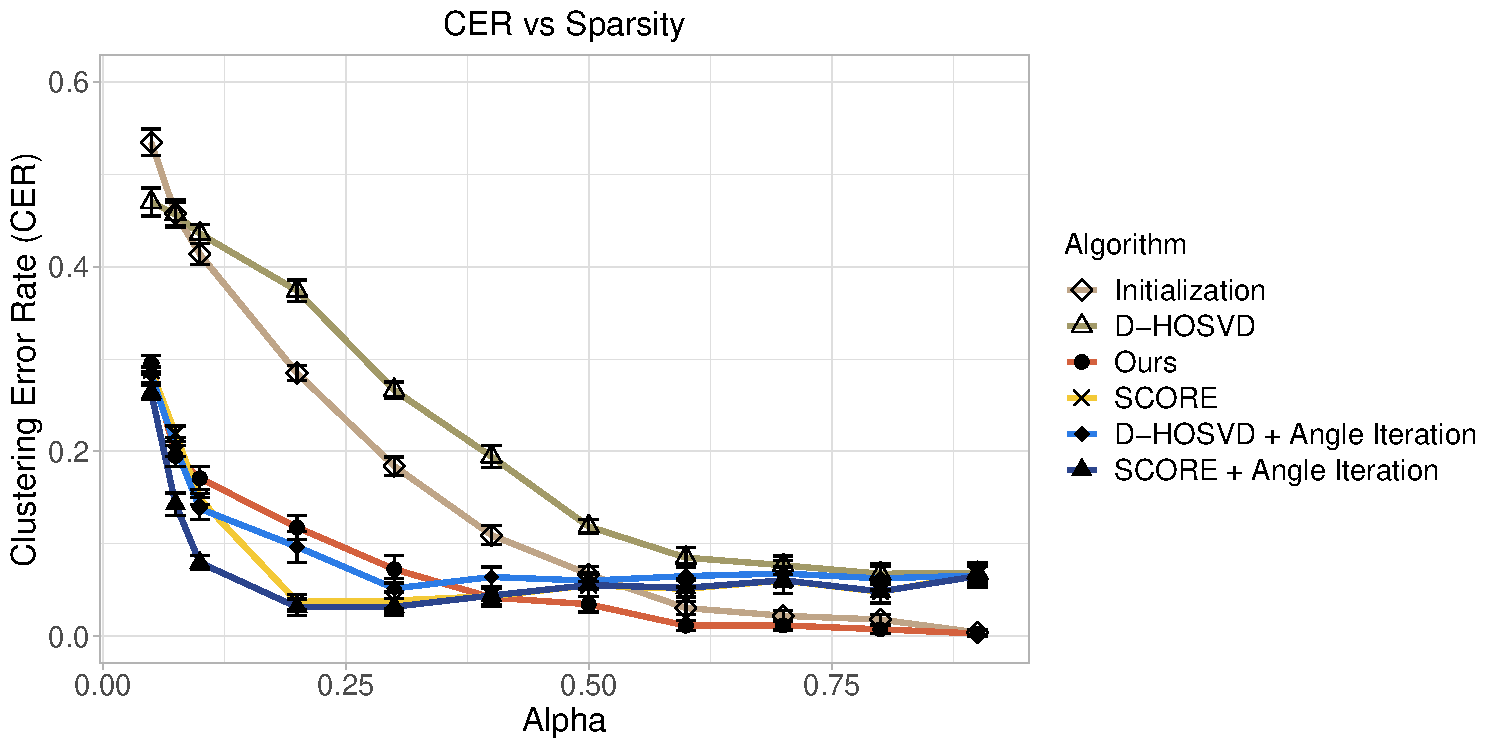
\includegraphics[width=.8\columnwidth]{sparsity.pdf}
    \caption{CER comparison versus sparsity parameter $\alpha_p$ in $[0.05, 0.9]$. We set $p = 100, r = 5$, and $\gamma = -1.2$ under sparse binary dTBM.}
    \label{fig:sparse}
\end{figure}

`` ...The second additional experiment evaluates the algorithm performances under the sparse binary dTBM~\eqref{eq:sparse_dtbm}. We fix the signal exponent $\gamma = -1.2$ and vary the sparsity parameter $\alpha_p \in [0.05, 0.9]$. A smaller $\alpha_p$ leads to a higher probability of zero entries in the observation. In addition to the three algorithms mentioned in Section~\ref{subsec:comp}  (denoted {\bf \small Initialization}, {\bf \small dTBM}, and {\bf \small SCORE}), we consider other three algorithms based on the discussion in Section~\ref{subsec:ber}: 
  \begin{itemize} 
  \item \textbf{\small D-HOSVD}, the diagonal-deleted HOSVD in \cite{ke2019community}; 
  \item \textbf{\small D-HOSVD + Angle}, the combined algorithm of our angle-based iteration with initialization from \textbf{\small D-HOSVD};
  \item \textbf{\small SCORE + Angle}, the combined algorithms of our angle-based iteration with initialization from \textbf{\small SCORE}.
  \end{itemize}
  
Figure~\ref{fig:sparse} shows a slightly larger error in \textbf{\small dTBM} than that in \textbf{\small SCORE}, \textbf{\small D-HOSVD + Angle}, and \textbf{\small SCORE + Angle} under the sparse setting with $\alpha_p < 0.3$. 
%The outperformance of \textbf{\small D-HOSVD} based iterative methods confirms the benefits of diagonal deletion in the sparse case. Meanwhile, 
The small gap between  \textbf{\small dTBM} and other sparse-specific methods implies the robustness of our algorithm. In addition, comparing \textbf{\small SCORE} versus \textbf{\small SCORE + Angle} (or \textbf{\small D-HOSVD} versus \textbf{\small D-HOSVD + Angle}) indicates the benefit of our angle iterations under the sparse dTBM. In the intermediate and dense cases with $\alpha_p \geq 0.3$, our proposed \textbf{\small dTBM} has a clear improvement over others, which again verifies the success of our algorithm in dense settings."
\end{quote}


\item \textit{ (Critical) The statistical lower bound is derived under non-degree TBM (since all $\theta(i) = 1$). From this, it is still not clear whether the lower bound would significantly increase when there is a skewed degree correction. The authors’ claim that the statistical lower bound matches MLE is difficult to verify (since I could not find an explicit result for MLE). Moreover, the stated upper bound (Thm 4-5) assume some uniformity in $\theta$ (see top of page-11), and so the (matched) upper/lower bounds could only be for the case of relatively homogeneous degrees. A more clear discussion on this would be useful. The present results leaves open the possibility that phase-transition SNR for dTBM could be arbitrarily worse than that of TBM, in which case making some assumption on balance is reasonable.}

\textbf{Response:}  

% \fixme{Miaoyan}{Say ``There seem to be three questions in this comments. We address them one by one. 
% \begin{enumerate}
% \item Regarding ``whether the lower bound would significatly increase when there is a skewed degree correction''. (move your response here)
% \item Regarding ``explicit result for MLE'' (move your response here)
% \item Regarding ``The stated upper bound assume some...''. 
% \end{enumerate}}

We thank reviewer for the suggestions. There seem to be three questions in this comment. We address them one by one.

\begin{enumerate}
    \item Regarding ``whether the lower bound would significantly increase when there is a skewed degree correction". We have revised the proof of statistical minimax bound with relaxed degree assumptions. Briefly, we relax the previous non-degree construction $\theta(i)\equiv 1$ to the skewed-degree construction under assumption~\eqref{eq:degree}. The latter allows moderate degree heterogeneity; for example, within each of the cluster, we allow the highest degree to be $\theta(i) = \Omega(p)$, whereas the lowest degree to be $\theta(i)=\tO(1)$. The revised minimax bound does not increase in the presence of moderately skewed degree. See our new Theorem~\ref{thm:stats} in Section~\ref{sec:limits} and new proof in Appendix II, Section~\ref{sec:statprove2}. 
    
       
    \item  Regarding ``explicit result for MLE". We have added the MLE guarantee in new Theorem~\ref{thm:stats}. The MLE error matches with statistical lower bound and ensures the dTBM achievability above the statistical critical value. We have also revised the exposure of Theorems~\ref{thm:stats}-\ref{thm:comp} to include both impossibility and achievability results. See our new Section~\ref{sec:statlimit} and Section~\ref{sec:complimit}. See our response to {\bf \# 2 Major Comments from Editor} for details.
    
    \item Regarding ``The stated upper bound assume some uniformity in $\theta$". We have added a new Section~\ref{sec:prelim} to discuss the rational for the balanced degree assumption~\eqref{eq:degree}. Briefly, we focus on the regime with balanced heterogeneity due to the relationship between dTBM performance and core tensor signal $\Delta_{\min}^2$. Indeed, without the balance assumption, the phase transition of dTBM can be arbitrarily worse than that of TBM. We quote our new discussion below:
    
New Section~\ref{sec:prelim}:
    \begin{quote}
    ``...In our work, we focus on the regime of balanced degree heterogeneity. We call the degree $\mtheta$ \emph{balanced} if
\begin{equation}\label{eq:degree}
{\min_{a\in[r]} \onormSize{}{\mtheta_{z^{-1}(a)}}=\left(1+o(1)\right)\max_{a\in[r]}\onormSize{}{\mtheta_{z^{-1}(a)}}}.
\end{equation}
The following lemma provides the rational of balanced degree assumption. We show the close relation between angle gaps in the mean tensor $\tX$ and the core tensor $\tS$ under balanced degree heterogeneity. 


\begin{lem}[Angle gaps in $\tX$ and $\tS$]\label{lem:angle_gap_x} Consider the dTBM model~\eqref{eq:model_tensor} under the parameter space $\tP$ in \eqref{eq:family}. Suppose Assumption~\ref{assmp:min_gap} holds and $\mtheta$ is balanced satisfying~\eqref{eq:degree}. Then, for all $i,j$ such that $z(i) \neq z(j)$, we have
\begin{equation}
 % \onorm{ \frac{\mX_{i:}}{\onormSize{}{\mX_{i:}}}  -  \frac{\mX_{j:}}{\onormSize{}{\mX_{j:}}}  } \asymp  \onorm{ \frac{\mS_{z(i):}}{\onormSize{}{\mS_{z(i):}}}  -  \frac{\mS_{z(j):}}{\onormSize{}{\mS_{z(j):}}}  },
 \cos(\mX_{i:}, \mX_{j:})\asymp  \cos(\mS_{z(i):}, \mS_{z(j):}),
\end{equation}

where $\mX =\mat(\tX)$ and $\mS = \mat (\tS)$.
\end{lem}

%Intuitively, the performance of dTBM is determined by both the core tensor and degree heterogeneity. Since we view degrees as nuisance parameters, our main interest is to characterize dTBM performance with respect to the signal $\Delta^2_{\min}$ in the core tensor. By Lemma~\ref{lem:angle_gap_x}, the mapping from the core tensor $\mS_{z(i):}$ to the mean tensor $\mX_{z(i):}$ preserves the angle information $\Delta_{\min}^2$ under balanced degree heterogeneity~\eqref{eq:degree}. Therefore, the balance assumption helps to exclude the cases in which the degree heterogeneity distorts the dTBM performance. 


In practice, an estimation algorithm has access to a noisy version of $\tX$ but not $\tS$. Our goal is to establish the algorithm performance with respect to the signal $\Delta^2_{\min}$ in the core tensor. By Lemma~\ref{lem:angle_gap_x}, the mapping from the core tensor $\mS_{z(i):}$ to the mean tensor $\mX_{z(i):}$ preserves the angle information $\Delta_{\min}^2$ under balanced degree heterogeneity~\eqref{eq:degree}. Therefore, the balanced degree assumption helps to exclude the cases in which the degree heterogeneity distorts the algorithm garantees. 

%Indeed, as we will see in Sections~\ref{sec:statlimit}-\ref{sec:complimit}, under the balance assumption~\eqref{eq:degree}, the $\Delta_{\min}^2$ is sufficient to establish the dTBM phase transition. 

%In contrast, a highly-skewed degree violating~\eqref{eq:degree} may lead to a worse performance of dTBM than that of TBM. 
Here, we provide an example to illustrate the insufficiency of $\Delta_{\min}^2$ in the absence of balanced degrees. 

% The balance assumption \eqref{eq:degree} ensures the sufficiency of core tensor signal $\Delta_{\min}^2$ to describe the phase transition of dTBM.
% Without balanced degree, 

%The dTBM phase transition without balanced degree may be arbitrary worse than that with balanced degree. 

\begin{example}[Insufficiency of $\Delta_{\min}^2$ in the absence of balanced degrees] Consider an order-2 $(p,p)$-dimensional dTBM with core matrix
\begin{equation}\label{eq:modelexample}
    \mS = \begin{pmatrix} 1 &a\\
    1 & -a
    \end{pmatrix}, \quad \text{and} \ \mtheta \text{ such that } \onormSize{}{\mtheta_{z^{-1}(1)}}^2 = p^m \onormSize{}{\mtheta_{z^{-1}(2)}}^2,
\end{equation}
where $m\geq 0$ is a scalar parameter controlling the skewness of degrees. Let $\Delta_{\mX}^2$ denote the angle gap of the mean tensor, defined by
\begin{equation}\label{eq:delta_x}
    \Delta_{\mX}^2 \coloneqq \min_{i,j \in [p], z(i) \neq z(j)} \onorm{ \frac{\mX_{i:}}{\onormSize{}{\mX_{i:}}}  -  \frac{\mX_{j:}}{\onormSize{}{\mX_{j:}}}  }, \quad \mX = \mat(\tX). %\quad  \tX = \tS \times_1 \mTheta \mM \times_2 \cdots \times_K \mTheta \mM.
\end{equation}
Take $ a = p^{-1/4}$ in the model setup~\eqref{eq:modelexample}. We have 
\begin{equation}
    \Delta_{\min}^2 = \frac{2 a^2}{1 + a^2} \asymp p^{-1/2}, \quad  \Delta_{\mX}^2 = \frac{2\onormSize{}{\mtheta_{z^{-1}(2)}}^{2} a^2}{\onormSize{}{\mtheta_{z^{-1}(1)}}^{2} +  \onormSize{}{\mtheta_{z^{-1}(2)}}^{2}a^2} \asymp p^{-1/2-m}.
\end{equation}
%Take $ a = p^{-1/4}. We have 
%\begin{equation}
   % \Delta_{\min}^2 = p^{-1/2} \quad \text{and} \quad    \Delta_{\mX}^2 = {1\over p^{m-1/2}+1} = \min(p^{1/2-m},1). 
    %{2 a^2 \over M+a^2} = p^{-1-\epsilon}.
%\end{equation}
% \begin{align}
%     &\text{if } a = p^{-1/2}, M = 1& \quad &\Rightarrow \quad \Delta_{\min}^2 =  \Delta_{\mX}^2 = p^{-1}; \\
%     &\text{if } a = p^{-1/4}, M = p^{1/2} & \quad &\Rightarrow \quad \Delta_{\min}^2 = p^{-1/2}, \   \Delta_{\mX}^2 = p^{-1}.
% \end{align}
%By the following Theorem~\ref{thm:stats}, no estimator achieves exact recovery of dTBM under $\Delta_{\mX}^2 < p^{-1}$. 
%Under the balanced degree assumption, the dTBM is computationally solvable based on our Theorem~\ref{thm:comp} in Section~\ref{sec:complimit}.
Based on our theory in later Sections, the stat-computational achievability of dTBM occurs when $\Delta^2_{\mX}>p^{-1}$; that is, the dTBM estimation depends on the relative magnitude of $m$ vs. $1/2$. In such a setting, the proposed signal notion $\Delta^2_{\min}$ alone fails to fully characterize dTBM. %However, the condition $ \Delta_{\min}^2 = p^{-1/2}$ with balanced degree leads to a computationally efficient dTBM by Theorem~\ref{thm:refinement}.
%$-1\leq \varepsilon \leq 1/2$.
 %($\tO(p^{-1}) \leq M \leq \tO(p)$ by the parameter space~\eqref{eq:family}). 
\end{example}

\begin{rmk}[Flexibility in balanced degree assumption] One important note is that our balance assumption~\eqref{eq:degree} does not preclude the mild degree heterogeneity. In fact, within each of the clusters, we allow the highest degree at the order $\tO(p)$, whereas the lowest degree at the order $\Omega(1)$. This range is more relaxed than previous work \citep{gao2018community} that restricts the highest degree in the sub-linear regime $o(p)$ and the lowest degree at the order $\Omega(1)$. 
\end{rmk}

\begin{rmk}[Similar assumptions in literature]
%We propose he balance assumption~\eqref{eq:degree} to avoid the extreme inflation or elimination of the core tensor gap $\Delta_{\min}^2$ after the weighted mapping by degree heterogeneity. 
Similar degree regulations are not rare in literature. In higher-order tensor model \citep{ke2019community}, the degree assumption $\max_{a\in[r]} \onormSize{}{\mtheta_{z^{-1}(a)}} \leq $ $ C \min_{a\in[r]}\onormSize{}{\mtheta_{z^{-1}(a)}}$ is made to ensure balancedness across communities. %Since they have no $\ell_1$ constraint on $\mtheta$, their balance assumption is equivalent to ours~\eqref{eq:degree} multiplying some constants to the degrees. " 
In \cite{gao2018community}, the degree distribution is restricted to ${1\over |z^{-1}(a)|}\sum_{i\in z^{-1}(a)}\theta_i=1+o(1)$ for all communities. 
\end{rmk}

    \end{quote}
    
\end{enumerate}

%Detailed revisions in Section~\ref{sec:limits} are in our response to \textbf{\# 2 Major Comments from Editor}. 

% For the statistical lower bound, we have revised the proof of minimax bound with general degree heterogeneity and the lower bound would not significantly increases. We have added the MLE guarantee to ensure the achievability above the statistical critical value. We have also revised the exposure of Theorem~\ref{thm:stats} and Theorem~\ref{thm:comp} to include both impossibility and achievability results. 

% We have changed the exposure of Theorems~\ref{thm:stats} and \ref{thm:comp} to include both the impossibility and achievement of dTBM problem when signal is below and above the critical values. We quote the revised paragraphs in Sections~\ref{sec:statlimit} and \ref{sec:complimit}.

%We focus on the regime with balanced $\mtheta$ due to our main interest on the relationship between dTBM performance and core tensor signal $\Delta_{\min}^2$. Indeed, without balance assumption, the phase transition of dTBM can be arbitrarily worse than that with balanced assumption or that of TBM. We have added a new Section~\ref{sec:prelim} to discuss the settings. \fixme{Miaoyan}{Quote your discussion here.}
% For the balance assumption on degree heterogeneity~\eqref{eq:degree}, we have added a preliminary section~\ref{sec:prelim} in Section~\ref{sec:limits} to discuss our signal notion and the balance regulation on $\mtheta$. The balance assumption is proposed to describe the performance of dTBM by the signal only in core tensor. We show an example to illustrate that the phase transition of dTBM would be arbitrary worse than TBM with unbalanced heterogeneity. Our statistical and computational limits are sharp under the regime of balance degree. We quote the discussion in the preliminary Section~\ref{sec:prelim} here:




% Our statistical lower bound is derived under the dTBM since we consider the estimator space without the equal degree assumption. The condition (i), $\theta(i) = 1$ for all $i \in [p]$, was assumed on true heterogeneity for technical convenience. We have now relaxed the equal degree condition (i) in the proof of Theorem 2 to avoid the ambiguity. We quote the revised proof below:

% \begin{quote}
%     ``
%     ... Specifically, we consider the estimation problem based on a particular parameter point $(\{z_k\}, \tS, \{\mtheta_k\})$ with the following two properties:
% \begin{equation}\label{eq:construction}
% \text{(i)}\ 
%     \Delta_{\min}\lesssim  \left({p\over r}\right)^{-\frac{K-1}{2}}\sigma; \quad  \text{(ii)}\ |z^{-1}_k(a)|={p \over r} \in \mathbb{Z}_+ \text{ for all }a\in[r],
% \end{equation}
% for all $k \in [K]$.

% Furthermore, we define a subset of indices $T_k \subset [p_k], k \in [K]$ in order to avoid the complication of label permutation. The construction of $T$ is precisely the same as \citet[Proof of Theorem 2]{gao2018community}. By the constraint $\onormSize{}{\mtheta_{z^{-1}(a)}}_1 = |z^{-1}(a)|, a \in [r]$ in parameter space (3), the $\max_{i \in T^c} \theta(i) \leq C$ for some positive constant $C$. Then, following the proof of~\citet[Theorem 2]{gao2018community}, ...."
% \end{quote}

% We have showed that MLE matches the statistical limit under the balance assumption in a new theorem. See our response to \textbf{\# 2 Major Comments from Editor.}

% \fixme{Jiaxin}{Need to rethink this question about the signal notion and phase transition.}
% {
% \color{red}

% The phase transition for dTBM is arbitrary worse than that of TBM, no matter with angle-based or Euclidean-based SNR. See Example 1. That's why we need to propose angle based SNR. 
% %To see the necessity of balance, we need to show the SNR phase transition will arbitrary worse than that with balance assumption. 


% Notice that 
% \begin{equation}
%     \{\text{$\mtheta$ is balanced} ,  \Delta_{\mS, \min}^2 \coloneqq \min \onormSize{}{\mS_{a:}^s - \mS_{b:}^s}^2 \leq p^{\gamma} \} \quad \subset \quad \{ \Delta_{\mA, \min}^2 \coloneqq \min \onormSize{}{\mA_{a:}^s - \mA_{b:}^s}^2 \leq  p^{\gamma}\},
% \end{equation}
% where $\mA = \mS (\mM^T \mTheta^T)^{\otimes K-1}$. 

% Our current statistical and computational limits are sharp under the former notion, $\Delta_{\mS, \min}^2$ with balance. The statistical lower bound and initialization guarantee still hold with latter notion $\Delta_{\mA, \min}^2$; but the computational limits, algorithm guarantees, MLE are not easy to extend with $\Delta_{\mA, \min}^2$.

% Specifically, in the computational lower bound,  we pick up a special example with $\theta = 1$. This special case lies in the parameter spaces generated by both signal notions. We apply Han's result to the special case, and this indicates computational lower bound can be much higher than current one; i.e., when $\Delta_{\mS, \min}^2$ with balance or $\Delta_{\mA, \min}^2 $ is larger than $p^{-K/2}$, it still may be computationally inefficient. The good news is: when $\Delta_{\mS, \min}^2 = p^{-K/2} \log p$ with balance, we have a polynomial time algorithm achieves exact recovery. Therefore, the threshold  $p^{-K/2}$ is sharp if we use the signal notion $\Delta_{\mS, \min}^2$ with balance.

%  In the iteration, we do not know the $\mtheta$ in practice, do not estimate $\tX$ in algorithm, and need the gap between folded vectors $\mS_{a:}$'s. Hence, it may not be easy to show the algorithm guarantee with later notion $\Delta_{\mA, \min}^2$; the MLE upper bound relies on iteration results  may also not be easy to extend.

% }


\item \textit{Please provide some intuition on Definition 2, particularly Eqn (10).}

\textbf{Response:} We have added more explanations for Definition~\ref{def:stable} and equation~\eqref{eq:local} in Section~\ref{subsec:angle}:
\begin{quote}
    ``... Roughly speaking, the vector $\mp(\bar z)$ represents the raw cluster sizes, and $\mp_\theta(\bar z)$ represents the relative cluster sizes weighted by degrees. ...The condition~\eqref{eq:local} controls the impact of node degree to the $\mp_{\theta}(\cdot)$ with respect to the misclassification rate $\varepsilon$ and angle gap $\Delta_{\min}$. Intuitively, the condition~\eqref{eq:local} controls the skewness of degree so that the angle between raw cluster size and degree-weighted cluster size is well controlled. The stability assumption is proposed for technical convenience, and we relax this condition in numerical studies; see Section~\ref{sec:simulation}."
\end{quote}

%We thank reviewer for the comment. Previous Definition 2 and equation (10) ensures the small gap between raw cluster size $|\hat z^{-1}(b)|$ and weighted cluster size $|\sum_{i \in \hat z^{-1}(b)} \theta(i)|$. With a better technique, we have shown the Definition 2 and the local linear stability condition on the heterogeneity $\mtheta$ are unnecessary for the algorithm guarantee. We have removed related parts from our manuscript.
\end{enumerate}

\newpage 
\begin{center}
    \textbf{Point-by-point Response to Reviewer 2}
\end{center}

\textit{Comments to the Author: This manuscript studies clustering under degree-corrected tensor block models (dTBMs). The dTBM is a generalization of the degree-corrected stochastic block model (DCSBM) for matrices/networks. It is also a generalization of the (non-degree) tensor block model (TBM) which is a higher-order extension of the stochastic block model (SBM).}

\textit{Contributions: The identifiability for the uniqueness of clustering under dTBMs is studied.
Statistical and computational lower bounds for clustering under dTBMs are established.
A two-stage, angle-based algorithm is proposed to achieve exact clustering in polynomial time under mild conditions. 
The last contribution is the most important one. The algorithm proposed uses the ``global-to-local strategy" which is commonly seen in community detection literature. An angle-based clustering is developed to handle the degree heterogeneity of dTBMs. Then theoretical analysis shows that it provably achieves the exact clustering. I feel this is a solid contribution, making the manuscript worth publication.} 

\textit{Nevertheless, I have a few concerns and comments.}

\begin{enumerate}[wide, labelwidth=!, labelindent=0pt]

\item \textit{One concern I have is that this manuscript is very similar to one of the authors' previous paper \cite{han2020exact} on clustering under the non-degree tensor block model. They share overall the same spirit, taste, and structure. For example:
The sessions for the computational and statistical lower bounds in this manuscript are very similar to the corresponding sessions in \cite{han2020exact} and they have the same results.
\cite{han2020exact} also gives a two-stage algorithm using the ``global-to-local strategy" and also achieves the exact clustering. \cite{han2020exact} gives the same threshold for the exact clustering as in this manuscript.
I think this manuscript should point out its connection with \cite{han2020exact}. The current version mentions that the method of \cite{han2020exact} fails under dTBMs but I think \cite{han2020exact} deserves more discussion given the similarity.}

\textbf{Response:} Thank you for your suggestion. We intentionally make the paper structure similar to~\cite{han2020exact} in order for easier comparison with non-degree models. Our results (e.g. the stat-comp lower bounds, the threshold for exact clustering) are all different from~\cite{han2020exact}. The confusion may come from the choice of our exposition: we chose the same notations as in~\cite{han2020exact} but actually they represent different quantities. 

We have added a new Section~\ref{sec:tbm}, ``Comparison with Non-degree Tensor Block Model'', to discuss the connection and difference between our dTBM work and TBM in \cite{han2020exact} from three aspects: signal notions, theoretical results, and algorithms. Please see our response to {\bf \# 1, Major Comments from Editor} for details. 


Briefly, we separate the discussion from three aspects: signal notion, theoretical results, and algorithm. We develop an angle-based signal notion to address the degree heterogeneity in dTBM. Our theoretical results are different with, and not easy extension of, the result in \cite{han2020exact}. Our algorithm share the classical local-to-global idea, but our angle-based iteration is specifically designed for dTBM and requires new proof techniques.  
%Particularly, our results in Section~\ref{sec:limits} are different with the result in \cite{han2020exact}. Though the critical values look the same, different signal notions lead to different interpretations of the results. The different parameter spaces and identifiability conditions also require different procedures to obtain the critical values. Also, our two-stage algorithm is different than that in \cite{han2020exact}. The angle-based update is specially designed for our degree-corrected model and brings a big challenge to establish the algorithm guarantee with polar coordinate based analysis. 



\item \textit{My next comment is about whether Session III B (computational lower bound) can be much simplified. My understanding is that the non-degree tensor block model is a special case of dTBMs, and hence lower bounds givens in \cite{han2020exact} also hold under dTBMs. As a result, I also feel the 2nd contribution this manuscript claim (ie, statistical and computational lower bounds) are relatively minor.}

\textbf{Response:} Thank you for your suggestion. The Session III B (computational lower bound) cannot be derived from earlier non-degree work~\citep{han2020exact}. The short answer is that, our results show the similar conclusion but {\bf under different conditions.} While the TBM impossibility~\citep{han2020exact} provides a necessary condition for our dTBM impossibility, we find that {\bf such a condition is loose} in our contexts. This has motivated to develop new techniques to derive sharp lower bounds. 

Inspired by your comment, we have revised the exposition of our theory. See our response to \textbf{\# 1 Major Comments from Editor} for details.

We quote the newly-added texts here:
\begin{quote}
    ``...\emph{Theoretical results.} In both works, we study the phase transition of TBM and dTBM with respect to the Euclidean and angle-based SNRs. We briefly summarize the results in \cite{han2020exact} and compare with ours. 
    
    \textit{Statistical critical value:}
    \begin{align}
        \text{Ours:}& \ \Delta_{\text{ang}}^2 \lesssim p^{-(K-1)} \Rightarrow \text{statistically impossible;} \quad \Delta_{\text{ang}}^2 \gtrsim   p^{-(K-1)} \Rightarrow \text{MLE achieves exact recovery;} \\
        \text{Han's:}& \ \Delta_{\text{Euc}}^2 \lesssim p^{-(K-1)} \Rightarrow \text{statistically impossible;} \quad \Delta_{\text{Euc}}^2 \gtrsim   p^{-(K-1)} \Rightarrow \text{MLE achieves exact recovery}.
    \end{align}
    
     \textit{Computational critical value:}
    \begin{align}
        \text{Ours:}& \ \Delta_{\text{ang}}^2 \lesssim p^{-K/2} \Rightarrow \text{computationally impossible;} \quad \Delta_{\text{ang}}^2 \gtrsim   p^{-K/2} \Rightarrow \text{ computationally efficient;} \\
        \text{Han's:}& \ \Delta_{\text{Euc}}^2 \lesssim p^{-K/2} \Rightarrow \text{computationally impossible;} \quad \Delta_{\text{Euc}}^2 \gtrsim   p^{-K/2} \Rightarrow \text{computationally efficient}.
    \end{align}
    
The above comparison reveals three major differences. 

 %Our dTBM phase transition re-discovers the statistical-computational gaps in TBM. %This finding indicates the intrinsic behavior distinctions among higher-order, matrix, and vector problem may be generally exists in many higher-order problems.
First, none of our results in Section~\ref{sec:limits} are corollaries of \cite{han2020exact}. Both models show the similar conclusion {\bf but under different conditions}. While the TBM impossibility~\citep{han2020exact} provides a necessary condition for our dTBM impossibility, we find that such a condition is often loose. There exists a regime of $\tS$ in which TBM problems are computationally efficient but dTBM problems are statistically impossible; see Example~\ref{example:euc_alg}. This observation has motivated us to develop the new signal notion $\Delta^2_{\text{ang}}$ for sharp dTBM phase transition conditions.  
     
 Second, to find the phase transition, we need to show both the impossibility {\bf and} achievability when SNR is below {\bf and} above the critical value, respectively. While the TBM impossibility can serve as a loose condition of our dTBM impossibility, more efforts are required to show the achievability. In particular, since TBM is a more restrictive model than dTBM, the achievability in \cite{han2020exact} does not imply the achievability of dTBM in a larger parameter space. The latter requires us to develop new MLE and polynomial algorithms for dTBM achievability.  %For impossibility, the minimax bounds in dTBM search over a larger range of estimators than TBM. Though the thresholds for TBM impossibility can serve as the loose lower bounds of the dTBM impossibility, more efforts are required to avoid the gap between impossibility and achievablity.
    
Third, from the perspective of proofs, we develop new tools to handle the extra degree heterogeneity. In our Theorem~\ref{thm:stats}, we consider the profile MLE by maximizing out the nuisance degree parameter, while TBM~\citep{han2020exact} considers the usual MLE without degree parameter. In our Theorem~\ref{thm:comp}, we construct a rank-2 tensor to relate HPC conjecture to $\Delta^2_{\text{ang}}$, while TBM~\citep{han2020exact} constructs a rank-1 tensor to relate HPC conjecture to $\Delta^2_{\text{Euc}}$. The asymptotic non-equivalence between $\Delta^2_{\text{ang}}$ and $\Delta^2_{\text{Euc}}$ renders our proof technically more involved...''
   \end{quote}
   
   \begin{quote}
   ``... \emph{Signal Notion.} We emphasize that the signal notions are different between the two models. In particular, the Euclidean-based signal notion in TBM~\cite{han2020exact} fails to accurately describe the phase transition in our dTBM due to the possible heterogeneity in degree $\mtheta$. To compare, we denote our angle-based signal notion in~\eqref{eq:gamma} and the Euclidean-based SNR in \cite{han2020exact} as $\Delta_{\text{ang}}^2$ and $\Delta_{\text{Euc}}^2$, respectively:
\begin{equation}
     \Delta_{\text{ang}}^2 =  2(1 - \max_{a \neq b\in [r]}\cos \of{\mS_{a:},\  \mS_{b:}} ), \quad \Delta_{\text{Euc}}^2 = \min_{a \neq b \in [r]} \onormSize{}{\mS_{a:} - \mS_{b:}}^2.
\end{equation}
By Lemma~\ref{lem:norm_diff} in the Appendix II, we have 
\begin{equation}\label{eq:signalcompare}
     \Delta_{\text{ang}}^2  \max_{a \in [r]}\onormSize{}{\mS_{a:}}^2 \leq \Delta_{\text{Euc}}^2.
\end{equation}
The above inequality indicates the condition $\Delta_{\text{Euc}}^2 \leq p^{\gamma}$ is {\bf sufficient but not necessary} for $\Delta_{\text{ang}}^2 \leq p^{\gamma}$. In fact, if we were to use $\Delta_{\text{Euc}}^2$ for both models, then the phase transition of dTBM can be arbitrarily worse than that for TBM. 


Here, we provide an example to illustrate the dramatical difference between TBM and dTBM with the same core tensor.  

\begin{example}[Comparison with Euclidean-based signal notion] \label{example:euc_alg} Consider a biclustering model with $\mtheta=1$ and an order-2 core matrix 
\begin{equation}
    \mS = \begin{pmatrix} p^{(\gamma+1)/2 } + 2  & 2 p^{(\gamma+1)/2} + 4\\
    2 & 4
    \end{pmatrix},\quad \text{with}\ \gamma \leq -1.
\end{equation}
The core matrix $\mS$ lies in the parameter spaces of TBM and our dTBM. Here, the constraint $\gamma \leq -1$ is added to ensure the bounded condition of $\mS$ in our parameter space in \eqref{eq:family}. The angle-based and Euclidean-based signal levels of $\mS$ are 
\begin{equation}
    \Delta_{\text{ang }}^2(\mS) = 0 \ \left(\leq p^{\gamma}\right), \quad \Delta_{\text{Euc}}^2(\mS) = 5 p^{\gamma + 1} \ \left(\geq p^{\gamma}\right).
\end{equation}
We conclude that TBM with $\mS$ achieves exact recovery with a polynomial-time algorithm; see \citet[Theorem 4]{han2020exact}. By contrast, the dTBM with the same $\mS$ and input $r=2$ violets the identifiability condition, and thus fails to be solved by all estimators; see our Theorem~\ref{thm:unique}.''
\end{example}

   \end{quote}
   We have revised our Section~\ref{sec:limits} to better present the lower bounds. See our response to \textbf{\# 1 Major Comments from Editor}. 



\item \textit{My third comment is on Condition (7), i.e., ``balance" of $\theta$. This is quite artificial and impractical and is needed only for technical reasons in the theoretical analysis of the proposed algorithm. In fact, as far as I know, this (or similar condition) is not needed in DCSBM literature for community detection. I suspect (7) can be removed by some better proof technique or modification of the proposed method.}

\textbf{Response:} Thank you for your suggestion. See our response to \textbf{\#3(a) and 3(c), Reviewer 1} (page 7 of this response letter) for the detailed response. 

While we agree the assumption is more for technical reasons, we suspect some ``balanced'' assumption or its variation seems necessary (and common in literature) for the achievability of computational critical values. 
Our constraints in $\tP$ are mild compared with previous literature. We have also added following comparison in Section~\ref{subsec:identify}:
\begin{quote}
    \begin{table}[h]
    \centering
    \resizebox{\textwidth}{!}{
    \begin{tabular}{c|c ccc}
    \hline
    Assumptions in parameter space& \cite{gao2018community}& \cite{han2020exact}& \cite{ke2019community} &Ours\\
    \hline
         Balanced community size &$\surd$ &$\surd$&$\surd$ & $\surd$  \\
        Balanced degree assumption & $\surd$&-&$\surd$ &$\surd$\\
         Bounded core tensor assumption & $\surd$ & $\times$ & $\surd$ &$\surd$\\
         Flexible in-group connections &$\times$ &$\surd$&$\surd$& $\surd$\\
         Gap among cluster centers & In-between cluster difference & Euclidean gap & Eigen gap & Angle gap\\
         \hline
    \end{tabular}
    }
    \caption{Parameter space comparison between previous work with our assumption.}
\end{table}


%We have added a new preliminary Section~\ref{sec:prelim} to discuss the regime with balanced $\mtheta$. The balance assumption is proposed to avoid the arbitrary bad phase transition of dTBM with respect to our signal notion. Similar regulations on degree also implicitly occur in DCSBM literature \cite{gao2018community, ke2019community}, in which more stringent constraints are applied on core tensor than ours. See our response to \textbf{ \# 3, Reviewer 1} for detailed discussion on balance assumption.

\end{enumerate}
\end{enumerate}


\newpage
\begin{center}
    \textbf{Point-by-point Response to Reviewer 3}
\end{center}

\textit{In general, this paper is well written and organized, numeric studies including simulation and real data application illustrate that the proposed model and method do have some merits. But I have several concerns regarding the theory and technical contribution.}

\begin{enumerate}[wide, labelwidth=!, labelindent=0pt]
\item \textit{Firstly, the mathematical formulation lacks motivation. From my knowledge, most existing degree-corrected block models are proposed for network data and Bernoulli model. While the proposed paper can be applied to Bernoulli as it could be taken as a special sub-Gaussian but I believe such treatment would not be suitable and/or optimal if one only cares about Bernoulli setting. Also, I notice several formulation inconsistencies. {For example, the author said they focus on symmetric tensor, but they assume the noise tensor $\mathcal{E}$ consists of independent entries, which does not make sense.}}



\textbf{Response:} Thank you for your suggestions. There seem to be three questions in this comment; we address them one-by-one. 

\begin{enumerate}
\item Regarding ``motivation of general sub-Gaussian model''.
Our proposal of sub-Gaussian dTBM is intended to cover multiple types of data in applications. Continuous tensors arise commonly in fields such as genetics and medical image studies. From theoretical perspective, our sub-Gaussian framework allows both binary and continuous observations. Conversely, binary-specific methods may not be suitable for general (continuous) sub-Gaussian data. %We have added a motivating example in Section~\ref{subsec:motiv} to emphasize the popularity of continuous data. 
%\begin{quote}
   % `` ...
    %\textit{Gaussian tensor mixture model:} The Gaussian mixture model is a common model in pattern recognition and image processing. We say an order-$K$ sample tensor $\tY \in \bbR^{p_1 \times \cdots \times p_K}$ follows a tensor Gaussian distribution with mean tensor $\tS \in \bbR^{p_1 \times \cdots \times p_K}$ if $\text{vec}(\tY)$ is a Gaussian vector with mean $\text{vec}(\tS)$. Tensor Gaussian mixture model assumes the tensor data $\tY_i$ for all $i \in [N]$ follow the mixture tensor Gaussian distribution with density $f(\tY_i) = \sum_{a = 1}^r \pi_a \phi_a(\tS_a), \quad i \in [N]$, where $r$ is the number of clusters, $\pi_a$ is the mixture weight, $\tS_a$ is the mean tensor, and $\phi_a$ denotes the tensor Gaussian density of the $a$-th cluster with mean $\tS_a$ for all $a \in [r]$. 

%Let $\tY \in \bbR^{N \times p_1 \times \cdots \times p_K }$ denote the combined data with slices $\tY(i,:) = \tY_i$ and $\tS \in \bbR^{r \times p_1 \times \cdots \times p_K}$ denote the combined mean tensor with slices $\tS(a,:) = \tS_a$. The tensor Gaussian mixture model with prior probability $\pi_a$ is equal to a special dTBM model
%\begin{equation}
   % \bbE[\tY] = \tS \times_1 \mM \times_2 \mI_{p_1} \times_3 \cdots \times_{K+1} \mI_{p_K},
%\end{equation}
%where $\mI_p$ is the identity matrix of dimension $p$, $\mM \in \{0,1\}^{N\times r}$ is the membership matrix for $N$ samples such that $\pi_a = |\{ i \in [N]: \mM_{i,a} = 1\} |/N$ for all $a \in [r]$. Assume that $\tS$ has a community structure. The tensor Gaussian mixture further becomes 
%\begin{equation}
   % \bbE[\tY] = \tC \times_1 \mM \times_2 \mTheta_1 \mM_1 \times_3 \cdots \times_{K+1} \mTheta_K \mM_K,
%\end{equation}
%where $\{ \mTheta_k, \mM_k\}_{k=1}^K$ refers to the heterogeneity and membership on the mean of Gaussian tensors. "
%\end{quote}


% First, our sub-Gaussian dTBM framework is well-motivated from the real life applications with multiple types of data. The general framework unifies a wide range of higher-order clustering models and facilities a comprehensive analysis for distinct observations. In contrast, the performances of existing Bernoulli methods are not guaranteed with general sub-Gaussian data. We have added more motivating examples to show and emphasize the importance of model flexibility. 
% {
% \color{blue}
% \begin{example}[Higher-order degree-corrected Gaussian mixture model] Gaussian mixture model is widely applied in applications including pattern recognition, image processing, and machine learning. We say an order-$K$ sample tensor $\tX \in \bbR^{p_1 \times \cdots \times p_K}$ follows a tensor Gaussian distribution with mean tensor $\tS \in \bbR^{p_1 \times \cdots \times p_K}$, denoted as $\tX \sim \tN(\tS; \mI_{p_1}, \ldots, \mI_{p_K})$, if $\text{vec}(\tY) \sim \tN( \text{vec}(\tS), \mI_{p_1 \cdots p_K})$, where $\mI_p$ is the identity matrix of dimension $p$.

% Higher-order degree-corrected Gaussian mixture model assumes the tensor data $\tY_i \in \bbR^{p_1 \times \cdots \times p_K}$ for all $i \in [N]$ follow the mixture tensor Gaussian distribution with density 
% \begin{equation} \label{eq:gaussian_mix}
%     f(\tY_i) = \sum_{a = 1}^r \pi_a \phi_a( \theta_i \tS_a; \mI_{p_1}, \ldots, \mI_{p_K}), \quad i \in [N],
% \end{equation}
% where $\theta_i$ is the heterogeneity of the $i$-th observation, $r$ is the number of clusters, $\pi_a$ is the mixture weight, $\tS_a$ is the mean tensor  and $\phi_a$ denotes the tensor Gaussian density of the $a$-th cluster, respectively, for all $r \in [a]$. 

% Let $\tY \in \bbR^{N \times p_1 \times \cdots \times p_K }$ denote the combined data with slices $\tY(i,:) = \tY_i$. Let $\tS \in \bbR^{r \times p_1 \times \cdots \times p_K}$ denote the combined mean tensor with slices $\tS(a,:) = \tS_a$. Further, we equip the mean tensor with community structure 
% \begin{equation}
%     \tS = \tC \times_2 \mM_1 \times_3 \cdots \times_{K+1} \mM_K,
% \end{equation}
% where $\tC \in \bbR^{r \times r_1 \times \cdots \times r_K}$ is the core tensor, and $\mM_k \in \{0,1\}^{p_k \times r_k}$ for all $k \in [K]$ are membership matrices. Consider the dTBM model
% \begin{equation}\label{eq:gaussian_mix_tbm}
%     \bbE[\tY] = \tC \times_1  \mTheta \mM \times_2 \mM_1 \times_3 \cdots \times_{K+1} \mM_K,
% \end{equation}
% where $\mTheta = \text{diag}(\theta_1, \cdots ,\theta_N)$ is the heterogeneity vector, $\mM \in \{0,1\}^{N \times r}$ is the membership matrix for $N$ samples. The higher-order degree-corrected Gaussian mixture model~\eqref{eq:gaussian_mix} is equivalent to our dTBM model~\eqref{eq:gaussian_mix_tbm} with prior probability $\pi_a = |\{ i \in [N]: \mM_{i,a} = 1\} |/N$ for all $a \in [r]$.
% \end{example}
% }
\item Regarding ``sub-optimality of Bernoulli as a special sub-Gaussian model''. We discuss below which of our results are still optimal for Bernoulli data, and which are not. 

\begin{itemize}
\item {\bf sub-Algorithm I.} Our initialization gaurantee is not suitable for Bernoulli data. To address this, we have proposed a remedy for Bernoulli initialization with square unfolding; see Section~\ref{subsec:ber}. The Bernoulli initialization error rate $\tO(p^{-\floor{K/2}})$ is slightly weaker than Gaussian initialization error rate $\tO(p^{-K/2})$. Combining the Bernoulli initialization with sub-Algorithm II, our method achieves an exponential error rate for Bernoulli data.
%and beats the state-of-art~\citep{ke2019community}. 

\item  {\bf sub-Algorithm II.} Our angle-based iteration guarantee is suitable for Bernoulli data. With Bernoulli data and a proper initialization, our iteration reduces the misclustering error from a polynomial rate to an exponential rate $\tO(\exp(-p^{K-1}))$, while the state-of-art algorithm for binary hypergraph \citep{ke2019community} leads to a polynomial error rate $\tO(p^{-2})$. 


\item {\bf Theorems~\ref{thm:stats}-\ref{thm:comp}.} The phase transitions are not applicable for Bernoulli data. The analyses of statistical phase transition and computational impossibility are based on Gaussian noise, and the polynomial-time algorithm achievability requires a larger SNR of order $\tO(p^{-\floor{K/2}})$ for Bernoulli data. We have added a numerical experiment in Appendix I to verify the existence of statistical-computational gap in Bernoulli tensor clustering. 
\end{itemize}

New Section~\ref{subsec:ber}: 
\begin{quote}
    ``...
    
    \textit{Initialization guarantee for Bernoulli data.} The main difficulty to establish the initialization guarantee for Bernoulli observations lies in the denoising step (lines 1-2 in Sub-algorithm~\hyperref[alg:main]{1}). We now provide a high-level explanation for the technical difficulty when applying Theorem~\ref{thm:initial} to Bernoulli observations. 
    
    
    The derivation of Theorem~\ref{thm:initial} relies on the upper bound of the estimation error for the mean tensor in Lemma~\ref{lem:two-step_esterror}; i.e., with high probability
\begin{equation}\label{eq:prop1}
    \onormSize{}{\hat \tX - \tX}_F^2 \lesssim p^{K/2},
\end{equation}
where $\tX = \bbE\tY$ and $\hat \tX$ is defined in Step 2 of Sub-algorithm~\hyperref[alg:main]{1}. Unfortunately, the inequality~\eqref{eq:prop1} holds only for i.i.d.\ sub-Gaussian observations, while Bernoulli observations are generally not identically distributed.  

One possible remedy is to apply singular value decomposition to the \emph{square unfolding}~\citep{mu2014square} of Bernoulli tensor $\tY$. We summarize the procedure in sub-algorithm 3.

\begin{algorithm}[h!]
\caption*{\bf Sub-algorithm 3: Weighted higher-order initialization for Bernoulli observation}
\vspace{.15cm}
\begin{algorithmic}[1] 
\INPUT Bernoulli tensor $\tY \in \{0,1\}^{p\times \cdots \times p}$, cluster number $r$, relaxation factor $\eta > 1$ in $k$-means clustering.
\State  Let the matrix $\mat_{sq} (\tY) \in \{0,1\}^{\floor{p^{K/2}} \times \ceil{p^{K/2}} }$ denote the nearly square unfolded tensor. Compute the estimate $\tX'$, where
\begin{equation}\label{eq:matrixsvd}
    \hat \tX' = \argmin_{\text{rank}(\mat_{sq}(\tX)) \leq r^{\ceil{K/2}}} \onormSize{}{ \mat_{sq}(\tX) -  \mat_{sq}(\tY)}_F^2.
\end{equation}
\State Implement lines 3-5 of Sub-algorithm~\hyperref[alg:main]{1} with $\hat \tX$ replaced by $\hat \tX'$ in~\eqref{eq:matrixsvd}.
\OUTPUT Initial clustering $z^{(0)} \leftarrow \hat z$.
\end{algorithmic}
\end{algorithm}

\begin{prop}[Error for Bernoulli initialization]\label{cor:ber} Consider the Bernoulli dTBM in the parameter space $\tP$ and Assumption~\ref{assmp:min_gap} holds. Assume that $\mtheta$ is balanced and $\min_{i\in[p]}\theta(i) \geq c$ for some constant $c>0$. Let $ z^{(0)}$ denote the output of Sub-algorithm~3. With probability going to 1, we have
\begin{equation}\label{eq:ini_b}
 \ell(z^{(0)}, z) \lesssim \frac{r^K p^{- \floor{K/2} }}{\text{SNR}}, \quad \text{and} \quad L(z^{(0)}, z) \lesssim  {\sigma^2 r^K p^{-\floor{K/2}}}.
\end{equation}
\end{prop}

\begin{proof}[Proof of Proposition~\ref{cor:ber}] Following Lemma 7 in \cite{gao2018community}, with high probability, the new estimate satisfies
\begin{equation}
    \onormSize{}{\hat \tX' - \tX}_F^2 \lesssim p^{\ceil{K/2}}.
\end{equation} 
We obtain the upper bound by using $\hat \tX'$ in place of $\hat \tX$  in Theorem~\ref{thm:initial}.
\end{proof}

\begin{rmk}[Comparison with previous methods] The Bernoulli bound $\tO(p^{- \floor{K/2} })$ in Proposition~\ref{cor:ber} is relatively looser than the Gaussian bound \tO(p^{- K/2 })$ in Theorem~\ref{thm:initial}. The gap between Bernoulli and Gaussian error decreases as the order $K$ increases. Nevertheless, combining with angle iteration Sub-algorithm~\hyperref[alg:main]{2}, Bernoulli clustering still achieves exponential error rate $\exp \of{ - p^{(K-1)}}$ at a price of a larger SNR.
%Nevertheless, the Bernoulli clustering still achieves exponential error rate $\exp \of{ - p^ \floor{K/2}}$ with large SNR combining with our angle iteration Sub-algorithm~\hyperref[alg:main]{2}. 
The exponential rate is tighter than the rate error $\tO(p^{-2})$ in previous work~\citep{ke2019community}. The investigation of the gap between upper bound $p^{- \floor{K/2}}$ and the lower bound $p^{- K/2}$ for Bernoulli tensors will be left as future work. In numerical experiments, we will use our original initialization, Sub-algorithm 1, to verify the robustness to Bernoulli observations."
\end{rmk}

\end{quote}

New Appendix I: 
\begin{quote}
   `` \textbf{Bernoulli phase transition.} The first additional experiment verifies the statistical-computational gap in Section~\ref{sec:limits} under the Bernoulli model. Consider the Bernoulli model with $p = \{80, 100\}$, $r = 5$. We vary $\gamma $ in $ [-1.2, -0.4]$ and $[-2.1, -1.4]$ for matrix ($K=2$) and tensor $(K = 3)$ clustering, respectively. We  approximate MLE using an oracle estimator, i.e., the output of Sub-algorithm~\hyperref[alg:main]{2} initialized from the true assignment. Figure~\ref{fig:phase_binary} shows a similar pattern as Figure~\ref{fig:phase}. The algorithm and oracle estimators have no gap in the matrix case, while an error gap emerges between the critical values $\gamma_{\text{stat}} = -2$ and $\gamma_{\text{comp}} = -1.5$ in the tensor case. Figure~\ref{fig:phase} suggests the statistical-computational gap in Bernoulli models."

\begin{figure}[htb]
    \centering
    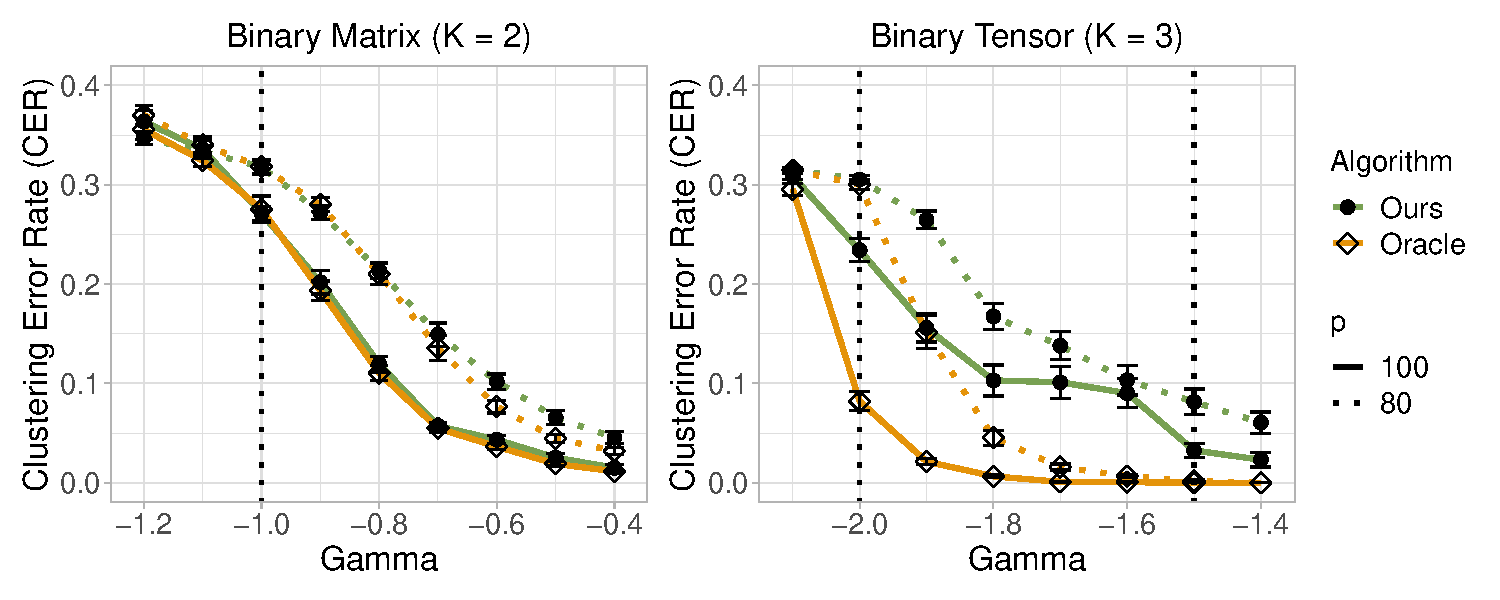
\includegraphics[width = .8\columnwidth]{binary_phase.pdf}
    \caption{SNR phase transitions for Bernoulli dTBM with $p = \{80, 100\}, r = 5$ under (a) matrix case with $\gamma \in [-1.2, -0.4]$ and (b) tensor case with $ \gamma \in [-2.1, -1.4]$.}
    \label{fig:phase_binary}
\end{figure}
\end{quote}

\item Regarding ``Formulation inconsistency". We agree that the original exposition is confusing and also unnecessary. We were attempting to simplify the notation by focusing on symmetric signal tensors (not necessarily symmetric data). Based on your comment, the revised paragraph in Section~\ref{sec:model} now reads

\begin{quote}
    ``... For ease of notation, we focus on the case with symmetric mean tensor $\bbE \tY$. This assumption simplifies the notation because all modes have the same $(\mTheta, \mM, z)$; the noise tensor $\tE$ and the data tensor $\tY$ are still possibly asymmetric. In general, we allow asymmetric mean tensor with $\{(\mTheta_k, \mM_k, z_k)\}_{k=1}^K$, one for each mode. The extension can be found in Appendix II...."
\end{quote}

In Section~\ref{sec:prelim}:
\begin{quote}
``...we provide...for general Gaussian dTBMs~\eqref{eq:model_margin} without symmetric assumptions. For general (asymmetric) Gaussian dTBMs, ....we extend the parameter space~\eqref{eq:family} to allow $K$ clustering functions $(z_k)_{k\in[K]}$, one for each mode. For notational simplicity, we still use $z$ and $\tP(\gamma)$ for this general (asymmetric) model. All results should be interpreted as the worst-case results across $K$ modes....''
\end{quote}

Consequently, we have revised our algorithm to reflect the asymmetry of data. We quote the revised algorithm in the last page of the response letter. We have also revised the notation in Theorems~\ref{thm:initial}-\ref{thm:refinement} by adding subscripts; that is, we now use $z_k^{(0)}$, $z_k^{(t+1)},\ldots$ in place of $z^{(0)}$, $z^{(t+1)}, \ldots$, throughout the paper.  

%\begin{quote}
   % \begin{thm}[Error for weighted higher-order initialization] Consider the general sub-Gaussian dTBM with i.i.d.\ noise under the parameter space $\tP$ and Assumption~\ref{assmp:min_gap}. Assume $\min_{i\in[p]}\theta(i) \geq c$ for some constant $c>0$ and let $\Delta_{\mX}$ denote the minimal gap in mean tensor defined in~\eqref{eq:delta_x}.  Let $ z^{(0)}_k$ denote the output of Sub-algorithm~\hyperref[alg:main]{1}. With probability going to 1, we have
%\begin{equation}
%    \ell(z^{(0)}_k, z) \lesssim {\sigma^2 r^K p^{-K/2}\over \Delta_{\mX}^2}.
%\end{equation}
%Further, assume $\mtheta$ is balanced as~\eqref{eq:degree}. We have
%\begin{equation}\label{eq:ini}
% \ell(z_k^{(0)}, z) \lesssim {r^K p^{-K/2}\over \text{SNR}} \quad \text{and} \quad L(z^{(0)}_k, z) \lesssim  {\sigma^2 r^K p^{-K/2}}
%\end{equation}
%\end{thm}


%\begin{thm}[Error for angle-based iteration] Consider the general sub-Gaussian dTBM with independent noise under the parameter space $\tP$ and Assumption~\ref{assmp:min_gap}. Let $\{z^{(0)}_k\}_{k=1}^K$ be the initialization for Sub-Algorithm~\hyperref[alg:main]{2} and $z^{(t)}_k$ be the $t$-th iteration output on $k$-th mode. Assume $\min_{i \in [p]}\theta(i) \geq c $ for some $c > 0$, the $\text{SNR} \geq \tilde C p^{-(K-1)}\log p$ for some sufficiently large constant $\tilde C$, and the initialization satisfies 
%\begin{equation}
%    L(z^{(0)}_k, z) \lesssim \frac{\Delta_{\min}^2}{r \log p}, \quad k \in [K].
%\end{equation}
%% With probability going to 1, there exists a contraction parameter $\rho \in (0,1)$ such that 
%\begin{align}\label{eq:final}
%    \ell(z, \hat z^{(t+1)}_k) \lesssim &\ \KeepStyleUnderBrace{
%   \text{SNR}^{-1}
%    \exp\of{- \frac{p^{K-1}\text{SNR}}{r^{K-1}}}}_{\substack{\text{statistical error}} }+ \KeepStyleUnderBrace{ \rho^t \ell(z, z^{(0)}_k). }_{\substack{\text{computational error}}}
%\end{align}
%\end{thm}

%\end{quote}



%Last, we have clarified the distribution of $\tE$ in equation~\eqref{eq:model_margin}. Throughout the paper, we consider the model with symmetric noise for simpler presentation; our theoretical results are based on the noise tensors with independent noise. We summarize the clarification here:
% \begin{quote}
%     ``..., and $\tE\in\mathbb{R}^{p\times \cdots \times p}$ is a symmetric noise tensor consisting of independent zero-mean sub-Gaussian entries $(i_1,\ldots, i_K)$ for indices $i_1 \leq \cdots \leq i_K$ with variance bounded by $\sigma^2$. The entries in $\tE$ satisfy  $\tE(i_1,\ldots,i_K) = \tE(\pi(i_1),\ldots,\pi(i_K))$ for any permutation $\pi$ on $\{i_1, \ldots, i_K\}$. The symmetric constraint in $\tE$ is relaxed for general dTBM. ..."
% \end{quote}
\end{enumerate}

\item \textit{I also found some technical assumptions strong.  For example, in Eq. (3), the authors restricted the matricization of core tensor has norm bounded from below and above. I don't see why that is necessary. The author argues ``...so the core tensor $\tS$ is not trivially reduced to a lower rank", but the tensor block model should be identifiable even when $\tS$ has degenerated rank. This leads to another question on the defined SNR in Eq. (4) (which requires minimal $\tS$ sliced norm). It is doubtful that this is a true quantity to work on.}

\textbf{Response:} This comment concerns the lower and upper bounds for the core tensor. We address them separately. 

\begin{enumerate}
\item Lower bound. Regarding ``...but tensor block model should be identifiable even when $\tS$ has degenerated rank.'' This is in fact what we intended to convey. Indeed, our remark of Theorem~\ref{thm:unique} reads: ``...the identifiability guarantee for the dTBM is stronger than classical Tucker model. .'' To avoid the confusion, we have revised the sentence into

\begin{quote}
``...Third, the lower bound constant $c_3>0$ requires no purely zero slide in $\tS$, and thus the model~\eqref{eq:model_tensor} is not trivially non-identifiable; see Example~\ref{example:c3}. 
...
\end{quote}

The lower boundness of core tensor slices is {\bf necessary} for the model identifiability. We have added following example in Section~\ref{subsec:identify} to illustrate the necessity of the lower bound $c_3$. 

\begin{quote}
    `` ...
    
    \begin{example}[Non-identifiability with purely zero core slice] Consider an order-2 dTBM with core tensor $\mS = \begin{pmatrix} 0 & 0\\
    1 & -1
    \end{pmatrix}$ and mean tensor 
    \begin{equation}
        \tX =  \mTheta_1 \mM \mS   \mM^T \mTheta_2, \quad \text{with } \mM = \begin{bmatrix} 1 & 0 \\
        1 & 0 \\
        0 & 1 \\
        0 & 1 \\
        \end{bmatrix}, \quad \mTheta_1 =\mTheta_2= \text{diag}(1,1,1,1).
    \end{equation}
Replacing $\mTheta_1$ by $\mTheta'_1 = (3/2, 1/2, 1,1)$ leads to the same mean tensor $\tX$. "
\end{example}
\end{quote}
We note that the purely zero slice in $\tS$ always makes the degree heterogeneity indistinguishable. Therefore, we exclude such case for model identifiability.

\item Upper bound. The upper bound $c_4>0$ is a technical constraint to avoid unbounded entries in the core tensor; in practices, the constraint $\max_{a\in[r]} \onorm{\mat(\tS)_{a:}} \leq c_4$ would likely never be active with a large choice of $c_4 \geq \onorm{\tY}$. We have changed the wording in Section~\ref{subsec:identify} into

\begin{quote}
    ``... The upper bound $c_4>0$ is a technical constraint to avoid unbounded entries in the core tensor. We introduce this assumption for proof convenience; in practical algorithms, the constraint $\max_{a\in[r]} \onorm{\mat(\tS)_{a:}} \leq c_4$ would likely never be active with a large choice of $c_4 \geq \onormSize{}{\tY}_F$. "
\end{quote}

\item Comparison of assumptions with previous work. Our constraints in $\tP$ are mild compared with previous literature. We have also added following comparison in Section~\ref{subsec:identify}:
\begin{quote}
    \begin{table}[h]
    \centering
    \resizebox{\textwidth}{!}{
    \begin{tabular}{c|c ccc}
    \hline
    Assumptions in parameter space& \cite{gao2018community}& \cite{han2020exact}& \cite{ke2019community} &Ours\\
    \hline
         Balanced community sizes &$\surd$ &$\surd$&$\surd$ & $\surd$  \\
         Bounded core tensors& $\surd$ & $\times$ & $\surd$ &$\surd$\\
              Balanced degrees & $\surd$&-&$\surd$ &$\surd$\\
         Flexible in-group connections &$\times$ &$\surd$&$\surd$& $\surd$\\
         Gaps among cluster centers & In-between cluster difference & Euclidean gap & Eigen gap & Angle gap\\
         \hline
    \end{tabular}
    }
    \caption{Parameter space comparison between previous work with our assumption.}
\end{table}
\end{quote}






% We agree that our dTBM is identifiable with some degenerated rank, and we thank the reviewer for pointing out the incorrect expression. The upper bound is technical constraint for theoretical analysis; in practice, the constraint $\max_{a:} \onorm{\mat(\mS)_{a:}} \leq c_4$ would likely never be active with a large $c_4 \geq \onorm{\tY}$.  Nevertheless, the lower bound of core tensor $\tS$ is still necessary for degree-corrected models. The lower bound is critical for identifiability; a purely zero slice in $\tS$ makes the heterogeneity indistinguishable. We have added a short counter-example to illustrate the necessity of non-zero core tensor slice.    

% {\color{blue}

% \begin{example}[Non-identifiability with pure zero core slice] Consider an order-2 dTBM with core tensor $\mS = \begin{pmatrix} 0 & 0\\
%     1 & -1
%     \end{pmatrix}$ and mean tensor 
%     \begin{equation}
%         \tX =  \mTheta_1 \mM \mS   \mM^T \mTheta_2, \quad \text{with } \mM = \begin{bmatrix} 1 & 0 \\
%         1 & 0 \\
%         0 & 1 \\
%         0 & 1 \\
%         \end{bmatrix}, \quad \mTheta_1 =\mTheta_2= \text{diag}(1,1,1,1).
%     \end{equation}
% Replacing $\mTheta_1$ by $\mTheta_1 = (3/2, 1/2, 1,1)$ leads to the same mean tensor $\tX$.
% \end{example}
% }

% In addition, the constraints in our parameter space are mild compared with previous degree-corrected block models \citep{gao2018community, ke2019community}. We have added a parameter space comparison table. 

% {
% \color{blue}

% \begin{table}[h]
%     \centering
%     \resizebox{\textwidth}{!}{
%     \begin{tabular}{c|c ccc}
%     \hline
%     Assumptions in parameter space& \cite{gao2018community}& \cite{han2020exact}& \cite{ke2019community} &Ours\\
%     \hline
%          Balanced community size &$\surd$ &$\surd$&$\surd$ & $\surd$  \\
%          Balanced degree parameters & $\surd$&-&$\surd$ &$\surd$\\
%          Bounded connection slices & $\surd$ & $\times$ & $\surd$ &$\surd$\\
%          Flexible in-group connections &$\times$ &$\surd$&$\times$& $\surd$\\
%          Gap among cluster centers & In-between cluster difference & Euclidean gap & Eigen gap & Angle gap\\
%          \hline
%     \end{tabular}
%     }
%     \caption{Parameter space comparison between previous work with our assumption.}
% \end{table}
% }

\end{enumerate}
\item \textit{Another big concern I have is the whole Section 3. The statistical and computational lower bounds are exactly the same as the tensor block model in \cite{han2020exact}. Therefore, the whole results in Section 3 can be simply obtained as corollary from \cite{han2020exact}. since the authors are working on a more restrictive model and the lower bounds must be larger than simpler model.}

\textbf{Response:} 

In fact, none of our results in Section 3 can be derived from earlier non-degree work~\citep{han2020exact}. The short answer is that, our results show the similar conclusion but {\bf under different conditions.} While the TBM impossibility~\citep{han2020exact} provides a necessary condition for our dTBM impossibility, we find that {\bf such a condition is loose} in our contexts. This has motivated to develop new techniques to derive sharp lower bounds. 
Inspired by your comment, we have revised the exposition of our theory. See our response to \textbf{\# 1 Major Comments from Editor} for details.

We quote the newly-added texts here:
\begin{quote}
    ``...\emph{Theoretical results.} In both works, we study the phase transition of TBM and dTBM with respect to the Euclidean and angle-based SNRs. We briefly summarize the results in \cite{han2020exact} and compare with ours. 
    
    \textit{Statistical critical value:}
    \begin{align}
        \text{Ours:}& \ \Delta_{\text{ang}}^2 \lesssim p^{-(K-1)} \Rightarrow \text{statistically impossible;} \quad \Delta_{\text{ang}}^2 \gtrsim   p^{-(K-1)} \Rightarrow \text{MLE achieves exact recovery;} \\
        \text{Han's:}& \ \Delta_{\text{Euc}}^2 \lesssim p^{-(K-1)} \Rightarrow \text{statistically impossible;} \quad \Delta_{\text{Euc}}^2 \gtrsim   p^{-(K-1)} \Rightarrow \text{MLE achieves exact recovery}.
    \end{align}
    
     \textit{Computational critical value:}
    \begin{align}
        \text{Ours:}& \ \Delta_{\text{ang}}^2 \lesssim p^{-K/2} \Rightarrow \text{computationally impossible;} \quad \Delta_{\text{ang}}^2 \gtrsim   p^{-K/2} \Rightarrow \text{ computationally efficient;} \\
        \text{Han's:}& \ \Delta_{\text{Euc}}^2 \lesssim p^{-K/2} \Rightarrow \text{computationally impossible;} \quad \Delta_{\text{Euc}}^2 \gtrsim   p^{-K/2} \Rightarrow \text{computationally efficient}.
    \end{align}
    
The above comparison reveals three major differences. 

 %Our dTBM phase transition re-discovers the statistical-computational gaps in TBM. %This finding indicates the intrinsic behavior distinctions among higher-order, matrix, and vector problem may be generally exists in many higher-order problems.
First, none of our results in Section~\ref{sec:limits} are corollaries of \cite{han2020exact}. Both models show the similar conclusion {\bf but under different conditions}. While the TBM impossibility~\citep{han2020exact} provides a necessary condition for our dTBM impossibility, we find that such a condition is often loose. There exists a regime of $\tS$ in which TBM problems are computationally efficient but dTBM problems are statistically impossible; see Example~\ref{example:euc_alg}. This observation has motivated us to develop the new signal notion $\Delta^2_{\text{ang}}$ for sharp dTBM phase transition conditions.  
     
 Second, to find the phase transition, we need to show both the impossibility {\bf and} achievability when SNR is below {\bf and} above the critical value, respectively. While the TBM impossibility can serve as a loose condition of our dTBM impossibility, more efforts are required to show the achievability. In particular, since TBM is a more restrictive model than dTBM, the achievability in \cite{han2020exact} does not imply the achievability of dTBM in a larger parameter space. The latter requires us to develop new MLE and polynomial algorithms for dTBM achievability.  %For impossibility, the minimax bounds in dTBM search over a larger range of estimators than TBM. Though the thresholds for TBM impossibility can serve as the loose lower bounds of the dTBM impossibility, more efforts are required to avoid the gap between impossibility and achievablity.
    
Third, from the perspective of proofs, we develop new tools to handle the extra degree heterogeneity. In our Theorem~\ref{thm:stats}, we consider the profile MLE by maximizing out the nuisance degree parameter, while TBM~\citep{han2020exact} considers the usual MLE without degree parameter. In our Theorem~\ref{thm:comp}, we construct a rank-2 tensor to relate HPC conjecture to $\Delta^2_{\text{ang}}$, while TBM~\citep{han2020exact} constructs a rank-1 tensor to relate HPC conjecture to $\Delta^2_{\text{Euc}}$. The asymptotic non-equivalence between $\Delta^2_{\text{ang}}$ and $\Delta^2_{\text{Euc}}$ renders our proof technically more involved...''
   \end{quote}
   
   \begin{quote}
   ``... \emph{Signal notion.} We emphasize that the signal notions are different between the two models. In particular, the Euclidean-based signal notion in TBM~\cite{han2020exact} fails to accurately describe the phase transition in our dTBM due to the possible heterogeneity in degree $\mtheta$. To compare, we denote our angle-based signal notion in~\eqref{eq:gamma} and the Euclidean-based SNR in \cite{han2020exact} as $\Delta_{\text{ang}}^2$ and $\Delta_{\text{Euc}}^2$, respectively:
\begin{equation}
     \Delta_{\text{ang}}^2 =  2(1 - \max_{a \neq b\in [r]}\cos \of{\mS_{a:},\  \mS_{b:}} ), \quad \Delta_{\text{Euc}}^2 = \min_{a \neq b \in [r]} \onormSize{}{\mS_{a:} - \mS_{b:}}^2.
\end{equation}
By Lemma~\ref{lem:norm_diff} in the Appendix II, we have 
\begin{equation}\label{eq:signalcompare}
     \Delta_{\text{ang}}^2  \max_{a \in [r]}\onormSize{}{\mS_{a:}}^2 \leq \Delta_{\text{Euc}}^2.
\end{equation}
The above inequality indicates the condition $\Delta_{\text{Euc}}^2 \leq p^{\gamma}$ is {\bf sufficient but not necessary} for $\Delta_{\text{ang}}^2 \leq p^{\gamma}$. In fact, if we were to use $\Delta_{\text{Euc}}^2$ for both models, then the phase transition of dTBM can be arbitrarily worse than that for TBM. 


Here, we provide an example to illustrate the dramatical difference between TBM and dTBM with the same core tensor.  

\begin{example}[Comparison with Euclidean-based signal notion] \label{example:euc_alg} Consider a biclustering model with $\mtheta=1$ and an order-2 core matrix 
\begin{equation}
    \mS = \begin{pmatrix} p^{(\gamma+1)/2 } + 2  & 2 p^{(\gamma+1)/2} + 4\\
    2 & 4
    \end{pmatrix},\quad \text{with}\ \gamma \leq -1.
\end{equation}
The core matrix $\mS$ lies in the parameter spaces of TBM and our dTBM. Here, the constraint $\gamma \leq -1$ is added to ensure the bounded condition of $\mS$ in our parameter space in \eqref{eq:family}. The angle-based and Euclidean-based signal levels of $\mS$ are 
\begin{equation}
    \Delta_{\text{ang }}^2(\mS) = 0 \ \left(\leq p^{\gamma}\right), \quad \Delta_{\text{Euc}}^2(\mS) = 5 p^{\gamma + 1} \ \left(\geq p^{\gamma}\right).
\end{equation}
We conclude that TBM with $\mS$ achieves exact recovery with a polynomial-time algorithm; see \citet[Theorem 4]{han2020exact}. By contrast, the dTBM with the same $\mS$ and input $r=2$ violets the identifiability condition, and thus fails to be solved by all estimators; see our Theorem~\ref{thm:unique}.'' 
\end{example}

   \end{quote}
   We have revised our Section~\ref{sec:limits} to better present the lower bounds. See our response to \textbf{\# 1 Major Comments from Editor}. 


\newpage


\begin{algorithm}[h!]
\caption*{\bf Algorithm: Multiway spherical clustering for degree-corrected tensor block model }
\vspace{.15cm}
\begin{algorithmic}[1]
\Algphase{Sub-algorithm 1: Weighted higher-order initialization}
\INPUT Observation $\tY \in \bbR^{p\times \cdots \times p}$, cluster number $r$, relaxation factor $\eta > 1$ in $k$-means clustering.

\State {
\color{blue}Compute factor matrix $ \mU_{\text{pre},k} = \text{SVD}_{r} (\text{Mat}_k(\tY)), k \in [K]$ and the $(K-1)$-mode projection 
\begin{equation}
    \tX_{\text{pre},k} = \tY \times_1   \mU_{\text{pre},1} \mU_{\text{pre},1}^T \times_2 \cdots  \times_{k-1} \mU_{\text{pre},k-1} \mU_{\text{pre},k-1}^T \times_{k+1} \mU_{\text{pre},k-1} \mU_{\text{pre},k+1}^T\times_{K+1}  \times_K \mU_{\text{pre},K} \mU_{\text{pre}, K}^T.
\end{equation}
}
\State {
\color{blue}
Compute factor matrix $\hat \mU_k = \text{SVD}_{r}(\text{Mat}_k(\tX_{\text{pre},k})), k \in [K]$ and denoised tensor
\begin{equation}
    \hat \tX = \tY \times_1 \hat \mU_1 \hat \mU^T_1 \times_2 \cdots \times_K \hat \mU_K \hat \mU^T_K.
\end{equation}
} 
\For{\textcolor{blue}{$k \in [K]$}}
\State { \color{blue} Let $\hat \mX = \text{Mat}_k(\hat \tX)$ and $S_0=\{i \in [p]: \onormSize{}{\hat \mX_{i:}} = 0\}$. Set $\hat z(i)$ randomly in $[r]$ for $i \in S_0$.}
\State{  For all $i\in S_0^c$, compute normalized rows
$\hat \mX_{i:}^s :=\onormSize{}{\hat \mX_{i:}}^{-1} \hat \mX_{i:}.$
}
\State { Solve the clustering $\hat z_k \colon [p]\to[r]$ and centroids $ (\hat \mx_j)_{j\in[r_k]}$ using weighted $k$-means, such that}
\begin{align}
    &\sum_{i \in S_0^c }  \onormSize{}{\hat \mX_{i:}}^2 \onormSize{}{\hat \mX_{i:}^s - \hat \mx_{\hat z_k(i)} }^2 
    \leq 
    \eta \min_{\substack{\bar \mx_j, j\in[r], \bar z_k(i),i\in S_0^{c}}} \sum_{i \in S^c } \onormSize{}{\hat \mX_{i:}}^2 \onormSize{}{ \hat \mX_{i:}^s -   \bar \mx_{\hat z_k(i)}}^2.
\end{align}
\EndFor

\OUTPUT {\color{blue} Initial clustering $z^{(0)}_k \leftarrow \hat z_k, k \in [K]$.}

\Algphase{Sub-algorithm 2: Angle-based iteration}
\INPUT Observation $\tY \in \bbR^{p \times \cdots \times p}$, initialization $z^{(0)}_k \colon [p]\to[r], k \in [K]$ from Sub-algorithm 1, iteration number $T$.
\For {$t = 0$ to $T-1$}
\State Update the block tensor $\tS^{(t)}$ via
$\tS^{(t)} (a_1,...,a_K)= \text{Ave} \{\tY(i_1,\ldots,i_K): z^{(t)}_k(i_k) = a_k, k \in [K]\}.$
\For{ $k \in [K]$}
\State {\color{blue} Calculate reduced tensor $\tY^{\text{d}}_k \in \bbR^{r \times r \times p \times r \times \cdots \times r}$ via
\begin{equation}
    \tY^{\text{d}}_k(a_1,\ldots,a_{k-1}, i ,a_{k+1},\ldots,a_K) 
    = \text{Ave}\{\tY(i_1,\ldots,i_{k-1},i,i_{k+1},\ldots,i_K): z^{(t)}(i_j) = a_j, j \neq k \}
\end{equation}}
% \begin{align}
%     &\tY^{\text{d}}(i,a_2,\ldots,a_K) 
%     = 
% \text{Ave}\{\tY(i,i_2,\ldots,i_K): z^{(t)}(i_k) = a_k, k \neq 1 \}.
% \end{align}

\State { \color{blue} Let $\mY_k^{\text{d}} = \text{Mat}_k(\tY^{\text{d}})$ and $J_0 = \{ i\in[p]: \onorm{\mY^{\text{d}}_{i:}} = 0\}$. Set $z_k^{(t+1)}(i)$ randomly in $[r]$ for $i \in J_0$.}

\State {\color{blue} Let $\mS^{(t)} = \text{Mat}(\tS^{(t)})$. For all $i \in J_0^c$ update the cluster assignment by
\begin{equation}
    z(i)^{(t+1)}_k = \argmax_{a \in [r]} \cos \left( \mY^{\text{d}}_{k,i:},\ \mS^{(t)}_{a:} \right).
\end{equation}}
\EndFor
\EndFor

\OUTPUT { \color{blue} Estimated clustering $z^{(T)}_k  \in [r]^{p}, k \in [K]$.}

\end{algorithmic}
\end{algorithm}

\end{enumerate}



% \begin{lem}[perturbation for degree-corrected clustering]. Let $z^*$ be the true clustering. Fix an arbitrary clustering $z$ with $\text{MisClust}(z,z^*):=\varepsilon \leq ...$ (a small constant). 
% Under assumptions....., we have
% \begin{equation}\label{eq:mode1}
% \min_{(\tS, \Theta)}\Fnorm{\tX(z^*, \tS^*, \Theta^*)-\tX(z; \tS, \Theta)}^2\gtrsim (...\text{factors involving $p^K$... }) \varepsilon \text{Angle-gap}^2 + o(\varepsilon).
% \end{equation}
% \end{lem}

% \begin{rmk}
% Everything is deterministic. Here, $\tX(z^*,...)$ is the degree-corrected signal tensor. Two ways to prove: 1) Find (deterministic)
% \[
% (\tS_{\min}, \Theta_{\min})=\argmin_{(\tS, \Theta)}\Fnorm{\tX(z^*)-\tX(z, \tS, \Theta)}^2,
% \]
% and then plug into~\eqref{eq:mode1} to evaluate the perturbation; 2) Prove a stronger version of identifiability result
% \[
% \KeepStyleUnderBrace{\min_{(\tS, \Theta, \tS^*, \Theta^*)}\Fnorm{\tX(z^*, \tS^*, \Theta^*)-\tX(z; \tS, \Theta)}^2}_{\text{distance between two points in the parameter space}}\gtrsim (...\text{factors involving $p^K$... })  \text{Angle-gap}^2 \KeepStyleUnderBrace{\varepsilon}_{\text{distance between $z$ and $z^*$}}.
% \]
% Our identifiability theorem is a special case of the above inequality by right hand side = 0.

% Lemma 1 is simpler than approaches in my NIPS paper, because no $\tY$ or expectation is needed. 
% In addition, I omitted the subscript $k$ in~\eqref{eq:mode1} for intuition. Precisely, ~\eqref{eq:mode1} holds only for $z_1$ while fixing $\{z_k\}_{k\geq 2}$. 
% \end{rmk}
% \begin{lem}[Union bound]
% \begin{align}
% &\mathbb{P}(\text{MisClust}(\hat z_{\text{MLE}}, z^*)\geq \varepsilon)\\
% \stackrel{\text{\color{red}You should write this step as instinct}}{=}&\mathbb{P}(\exists (z, \tS, \Theta) \ \text{s.t.}\  \text{MisClust}(z,z^*)\geq \varepsilon \ \text{and}\ \text{Log-lik}(z, \tS, \Theta) \geq \text{Log-lik}(z^*))\\
% %&\leq \sum_{z \text{ for which MisClust}(z,z^*)\geq \varepsilon}\mathbb{P}(\text{Log-lik}(z)\geq \text{Log-lik}(z^*))\\
% \leq &\sum_{z \text{ for which MisClust}(z,z^*)\geq \varepsilon}\sum_{(\tS, \Theta)}\mathbb{P}(\Fnorm{\tY-\tX(z, \tS, \Theta)}^2\leq \Fnorm{\tY-\tX(z^*)}^2)\\
% \leq & \sum_{z:\ \text{MisClust}(z,z^*)\geq \varepsilon}\sum_{(\tS, \Theta)} \mathbb{P}\left({\langle \tE, \tX(z^*)-\tX(z, \tS, \Theta)\rangle  \over\Fnorm{\tX(z^*)-\tX(z, \tS, \Theta)}}\gtrsim \Fnorm{\tX(z^*)-\tX(z, \tS, \Theta)} \right)\\
% \leq& \text{(desired conclusion)}
% \end{align}


% In the last step, only randomness is on $\tE$. The term $\Fnorm{\tX(z^*)-\tX(z,...)}$ can be replaced by $...\sqrt{\varepsilon}$ because of condition in the sum ``$z$ for which MisClust$(z,z^*)\geq \varepsilon$ '' and Lemma 1. 
 
% \fixme{Miaoyan}{Please complete full steps using ideas from Lemma 1 and Thm 1 in my NIPS paper. Lemma 2 is simple. I sketched out the proof for Lemma 1 for $R=2$. For general $R$ (number of blocks), it should be doable (I did not do) with just more notations}


% \end{lem}

\bibliography{tensor_wang}
\bibliographystyle{apalike}

\end{document}
 